%% ----------------------------------------------------------------
%% Project.tex
%% ---------------------------------------------------------------- 
\documentclass{ecsproject}     
\usepackage[backend=bibtex8, style=ieee]{biblatex}
\usepackage{acro}
\usepackage[singlelinecheck=false]{caption}
\usepackage{booktabs}
\usepackage{float}
\usepackage{makecell}
\usepackage{subfig}
\usepackage{pgfgantt}
\usepackage{longtable}
\usepackage[shortlabels]{enumitem}
\usepackage{array}
\usepackage{multirow}
\usepackage{colortbl}
\usepackage[math]{cellspace}
\usepackage{amsmath}
\usepackage[edges]{forest}

\newcommand{\PreserveBackslash}[1]{\let\temp=\\#1\let\\=\temp}
\newcolumntype{C}[1]{>{\PreserveBackslash\centering}m{#1}}
\newcolumntype{R}[1]{>{\PreserveBackslash\raggedleft}m{#1}}
\newcolumntype{L}[1]{>{\PreserveBackslash\raggedright}m{#1}}
\newcommand{\centered}[1]{\begin{tabular}{l} #1 \end{tabular}}

\input{Definitions}
% class `abbrev': abbreviations:
\DeclareAcronym{lora}{
  short = LoRa,
  long  = \textbf{Lo}ng \textbf{Ra}nge (radio) ,
  class = abbrev
}

\DeclareAcronym{phy}{
  short = PHY,
  long  = \textbf{Phy}sical Layer,
  class = abbrev
}

\DeclareAcronym{csma}{
  short = CSMA,
  long  = \textbf{C}arrier-\textbf{s}ense \textbf{M}utliple \textbf{A}ccess,
  class = abbrev
}

\DeclareAcronym{macaw}{
  short = MACAW,
  long  = \textbf{M}ultiple \textbf{A}ccess with \textbf{C}ollision \textbf{A}voidance (for \textbf{W}ireless LANs),
  class = abbrev
}

\DeclareAcronym{pc}{
  short = PC,
  long  = \textbf{P}acket \textbf{C}ount,
  class = abbrev
}

\DeclareAcronym{dc}{
  short = DC,
  long  = \textbf{D}uty \textbf{C}ycle,
  class = abbrev
}


\DeclareAcronym{dr}{
  short = DR,
  long  = \textbf{D}ata \textbf{R}ate,
  class = abbrev
}

\DeclareAcronym{eh}{
  short = EH,
  long  = \textbf{E}xplicit  \textbf{H}eader,
  class = abbrev
}

\DeclareAcronym{prp}{
  short = PRP,
  long  = \textbf{P}acket \textbf{R}eceive \textbf{P}ercentage,
  class = abbrev
}

\DeclareAcronym{mac}{
  short = MAC,
  long  = \textbf{M}edium \textbf{A}ccess \textbf{C}ontrol,
  class = abbrev
}

\DeclareAcronym{dap}{
  short = DAP,
  long  = \textbf{D}ata \textbf{A}nnouncement \textbf{P}acket,
  class = abbrev
}

\DeclareAcronym{llbp}{
  short = LLBP,
  long  = \textbf{L}oRa \textbf{L}ocal \textbf{B}roadcast \textbf{P}rotocol,
  class = abbrev
}

\DeclareAcronym{td}{
  short = TD,
  long  = \textbf{T}est \textbf{D}efinition,
  class = abbrev
}

\DeclareAcronym{fspl}{
  short = FSPL,
  long  = \textbf{F}ree \textbf{S}pace \textbf{P}ath \textbf{L}oss,
  class = abbrev
}

\DeclareAcronym{pe}{
  short = PE,
  long  = \textbf{P}lain \textbf{E}arth,
  class = abbrev
}

\DeclareAcronym{sp}{
  short = SP,
  long  = \textbf{S}lave \textbf{P}osition,
  class = abbrev
}

\DeclareAcronym{mp}{
  short = MP,
  long  = \textbf{M}aster \textbf{P}osition,
  class = abbrev
}

\DeclareAcronym{ps}{
  short = PS,
  long  = \textbf{P}reamble \textbf{S}ymbol,
  class = abbrev
}

\DeclareAcronym{rps}{
  short = RPS,
  long  = \textbf{R}eceived \textbf{P}acket \textbf{S}trength,
  class = abbrev
}

\DeclareAcronym{los}{
  short = LOS,
  long  = \textbf{L}ine \textbf{o}f \textbf{S}ight,
  class = abbrev
}

\DeclareAcronym{olsr}{
  short = OLSR ,
  long  = \textbf{O}ptimised \textbf{L}ink \textbf{S}tate \textbf{R}outing (protocol),
  class = abbrev
}

\DeclareAcronym{lar}{
  short = LAR ,
  long  = \textbf{L}ocation \textbf{A}ided \textbf{R}outing (protocol),
  class = abbrev
}

\DeclareAcronym{aodv}{
  short = AODV ,
  long  = \textbf{A}d-Hoc \textbf{O}n \textbf{D}emand Distance \textbf{V}ector (protocol),
  class = abbrev
}

\DeclareAcronym{dtn}{
  short = DTN,
  long  = \textbf{D}elay \textbf{T}olerant \textbf{N}etwork ,
  class = abbrev
}

\DeclareAcronym{scf}{
  short = SCF,
  long  = \textbf{S}tore \textbf{C}arry \textbf{F}orward ,
  class = abbrev
}

\DeclareAcronym{rf}{
  short = RF,
  long  = \textbf{R}adio \textbf{F}requency,
  class = abbrev
}

\DeclareAcronym{crc}{
  short = CRC,
  long  = \textbf{C}yclic \textbf{R}edundancy \textbf{C}heck,
  class = abbrev
}

\DeclareAcronym{adr}{
  short = ADR,
  long  = \textbf{A}daptive \textbf{D}ata \textbf{R}ate,
  class = abbrev
}

\DeclareAcronym{psa}{
  short = PSA,
  long  = \textbf{P}olite \textbf{S}pectrum \textbf{A}ccess,
  class = abbrev
}

\DeclareAcronym{eirp}{
  short = EIRP,
  long  = \textbf{E}quivalent \textbf{I}sotropically \textbf{R}adiated \textbf{P}ower,
  class = abbrev
}

\DeclareAcronym{fcc}{
  short = FCC,
  long  = \textbf{F}ederal \textbf{C}ommunications \textbf{C}ommission,
  class = abbrev
}

\DeclareAcronym{dsss}{
  short = DSSS,
  long  = \textbf{D}irect \textbf{S}equence \textbf{S}pread \textbf{S}pectrum,
  class = abbrev
}

\DeclareAcronym{srd}{
  short = SRD,
  long  = \textbf{S}hort \textbf{R}ange \textbf{D}evice,
  class = abbrev
}


\DeclareAcronym{etsi}{
  short = ETSI,
  long  = \textbf{E}uropean \textbf{T}elecommunications \textbf{S}tandards \textbf{I}nstitute,
  class = abbrev
}


\DeclareAcronym{manet} {
  short = MANET ,
  long  = \textbf{M}obile \textbf{A}d-hoc \textbf{Net}work ,
  class = abbrev
}

\DeclareAcronym{lpwan}{
  short = LPWAN ,
  long  = \textbf{L}ow \textbf{P}ower \textbf{W}ide \textbf{A}rea \textbf{N}etwork,
  class = abbrev
}

\DeclareAcronym{lan}{
  short = LAN ,
  long  = \textbf{L}ocal \textbf{A}rea \textbf{N}etwork,
  class = abbrev
}

\DeclareAcronym{wan}{
  short = WAN ,
  long  = \textbf{W}ide \textbf{A}rea \textbf{N}etwork,
  class = abbrev
}

\DeclareAcronym{lte}{
  short = LTE ,
  long  = \textbf{L}ong-\textbf{T}erm \textbf{E}volution,
  class = abbrev
}

\DeclareAcronym{css}{
  short = CSS ,
  long  = \textbf{C}hirp \textbf{S}pread \textbf{S}pectrum,
  class = abbrev
}

\DeclareAcronym{sf}{
  short = SF ,
  long  = \textbf{S}preading \textbf{F}actor,
  class = abbrev
}

\DeclareAcronym{bw}{
  short = BW ,
  long  = \textbf{B}and\textbf{w}idth,
  class = abbrev
}

\DeclareAcronym{cr}{
  short = CR ,
  long  = \textbf{C}oding \textbf{R}ate,
  class = abbrev
}
\DeclareAcronym{ism}{
  short = ISM ,
  long  = {\textbf{I}ndustrial, \textbf{S}cience, Medical} ,
  class = abbrev
}

\DeclareAcronym{fec}{
  short = FEC ,
  long  = {\textbf{F}orward \textbf{E}rror \textbf{C}orrection} ,
  class = abbrev
}

\DeclareAcronym{cad}{
  short = CAD,
  long  = {\textbf{C}hannel \textbf{A}ctivity \textbf{D}etection} ,
  class = abbrev
}

\DeclareAcronym{rssi}{
  short = RSSI ,
  long  = \textbf{R}eceived \textbf{S}ignal \textbf{S}trength \textbf{I}ndication,
  class = abbrev
}
\DeclareAcronym{snr}{
  short = SNR ,
  long  = {\textbf{S}ignal-\textbf{N}oise-\textbf{R}atio} ,
  class = abbrev
}

\DeclareAcronym{per}{
  short = PER ,
  long  = {\textbf{P}acket \textbf{E}rror \textbf{R}ate} ,
  class = abbrev
}

\DeclareAcronym{ber}{
  short = BER ,
  long  = {\textbf{B}it \textbf{E}rror \textbf{R}ate} ,
  class = abbrev
}

\DeclareAcronym{cf}{
  short = CF ,
  long  = {\textbf{C}arrier \textbf{F}requency} ,
  class = abbrev
}

\DeclareAcronym{pl}{
  short = PL ,
  long  = {\textbf{P}acket \textbf{L}ength} ,
  class = abbrev
}

\DeclareAcronym{tp}{
  short = TP ,
  long  = {\textbf{T}ransmit \textbf{P}ower} ,
  class = abbrev
}

\DeclareAcronym{lorawan}{
  short = LoRaWAN ,
  long  = {\textbf{Lo}ng \textbf{Ra}nge \textbf{W}ide \textbf{A}rea \textbf{N}etwork} ,
  class = abbrev
}

\DeclareAcronym{rtc}{
  short = RTC ,
  long  = {\textbf{R}eal \textbf{T}ime \textbf{C}lock} ,
  class = abbrev
}
\DeclareAcronym{lipo}{
  short = Li-Po,
  long  = \textbf{Li}thium \textbf{Po}lymer (battery),
  class = abbrev
}

\graphicspath{{../Figures/}}
\hypersetup{colorlinks=false}
\acsetup{first-style=short}
\bibliography{citations}

%% ----------------------------------------------------------------
\begin{document}
\frontmatter
\title      {LoRa Communications for Sparse Robot Swarms}
\authors    {\texorpdfstring
             {\href{mailto:dsj1n15@soton.ac.uk}{David Jones}}
             {David Jones}
            }
\addresses  {\groupname\\\deptname\\\univname}
\date       {\today}
\subject    {}
\keywords   {}
\supervisor {Dr Klaus-Peter Zauner}
\examiner   {Prof. Kirk Martinez}
\degree     {MEng Computer Science}
\maketitle

\begin{abstract}
 

\end{abstract}

\tableofcontents
\listoffigures
\listoftables
%\lstlistoflistings


\chapter{Acronyms}
\vspace{-20mm}
\printacronyms[include-classes=abbrev, name=]
\printacronyms[include-classes=radio_params, name=]

\input{Symbols}
\acknowledgements{
This work would not have been possible without Klaus Peter-Zauner's weekly guidance and continuous support. I am also thankful to Kirk Martinez for his invaluable suggestions on simulation methods, which kept this project progressing. Most of all I would like to thank any family and friends who kept me company through the many hours of data collection, no matter the weather!
}
\mainmatter

%% ----------------------------------------------------------------
\chapter{Introduction}
Decentralisation of wireless control and data sharing systems allows flexible deployment structures over large areas. Conversely, using a single centralised node, deployments are limited by that node's placement and its maximum communication range. This paper studies the application of \ac{lora}, an emerging long range, low power, radio frequency (\ac{rf}) technology, for the decentralised use case of sparse robot swarms. Solutions are targeted at, and scenarios are devised from, the use case, however as the research topics discussed are applicable to many areas, descriptions are largely kept agnostic. 
  
Swarm robotics is the coordination of multi-robot systems such that a common goal can be achieved. Capabilities of a swarm should exceed that of any single robot in the swarm; be that attributed to increased coverage \cite{Ducatelle:2011:Pathfinding} or self-assembly methods \cite{3YP:OBSTACLE_SWARMS}. Although spreading robots across large areas opens up potential for many practical applications, including terrain mapping, and search and rescue, the sophistication of robots required in these real-world scenarios can make them prohibitively expensive, which can lead to limited robot density. These are referred to as sparse swarms.
 
Unlike a centralised control approach, swarms rely on robots sharing data directly so that all instances can build a combined interpretation of the environment. Although some data may need to be decimated to many or all robots in the network for purposes such as swarm management, the vast majority will only be of interest to physically local neighbours. Local interest data may be found obstacles or robot routes. In critical scenarios, for example when robot failure is impending, large fast data dumps may be required. Alternatively, data can be continuously aggregated and distributed in a BitTorrent-like fashion \cite{3YP:SOUL}.
%Global interest data may be for swarm management, e.g. voting decisions, or be generic, e.g. battery usage figures for specific terrain fingerprints. 

For concentrated deployments, these scenarios are trivial to implement using high-data-rate technologies such as Wi-Fi. However, in a real-world scenario, when inter-robot distance is significant, and there are line of sight (\ac{los}) obstructions (e.g. trees), an alternative physical medium is required. This leads to the choice of \ac{lora}, detailed in Section \ref{sec:lora}. The system can be considered as a mobile-ad-hoc-network (\ac{manet}), due to the ever changing topology caused by internal system changes (e.g. robot movement), or external system changes (e.g. weather).

Although \ac{lora} is fundamentally ideal for long-range applications and operates in the low attenuation Sub-1GHz band, scenario specific conditions of ground-level transmissions and high-propagation environments are not ideal for \ac{rf} communications. Therefore this project initially covers real-world testing in free-space and forests to assess how sparse swarm deployment scenarios may affect \ac{lora}'s physical radio performance. From this, demodulation models are extracted and combined with \ac{lora} collision models from literature to create a simulator for testing \ac{lora} ad-hoc scenarios. This simulator is used to analyse the effectiveness of three \ac{mac} protocols with the aim of distributing local-interest data to physically local neighbours. Two methods utilise common approaches (ALOHA and \ac{csma}), and the third attempts to exploit hardware parameters and regional \ac{rf} regulations; this is defined as the LoRa Local Broadcast Protocol (\ac{llbp}).

%Alongside the physical communication medium, a  is needed.
%Many MAC layer protocols exist 
%\cite{3YP:FLOCK_1, 3YP:FLOCK_2, 3YP:FLOCK_3}
%Separation distance is less of an issue as much existing work covers guaranteeing minimum connectivity via positioning !!!.

%Power usage must be proportionate to that of the overall robot,  i.e. power usage can exceed that of nodes in a fixed-position sensor network but not extend to long range Wi-Fi. In a real-world scenario the communications must be robust to physical environmental changes, which can stem from circumstances that are either external to the system, such as weather, or internal to the system, such as robot positioning. The latter having resulting factors such as varying separation distance or change in line of sight propagation caused by obstacles (e.g. trees and ridges). Wi-Fi signals in the 2.4GHz or 5GHz bands are easily attenuated so an alternative physical medium is required; this leads to the choice of \ac{lora}, which operates in the Sub-1GHz band.

%If radio hardware is designed for a worst case scenario, the throughput for normal situations will ve greatly impaired. If the hardware is designed for an average situation. the network risks partition under stress because of poor radio links.

%The target should be to minimise airtime. Longer airtime increases collision chance and reduces throughput of the network as a whole.
\chapter{Background}
\section{\ac{lora}}
\label{sec:lora}
\subsection{Overview}
\ac{lora} is a physical long-range, low-power, communication technology developed and patented by Semtech\footnote{Semtech, USA, https://www.semtech.com/}. It is designed to operate inside either the Sub-1GHz or 2.4GHz unlicensed \ac{ism} bands worldwide. Consequently, under the proviso that local regulatory standards are obeyed (see Section \ref{sec:ISMBandRegulation}), it can be used for wide area deployments without being tied to expensive licensed carriers. Fundamentally, even using its fastest configuration, it is a low-data rate modulation technique.

Long-range communication can be a challenge in the \ac{ism} bands as the heavy congestion can result in a high physical noise floor. That is the sum of all signals in the band from sources such as the atmosphere or radio devices, excluding that of the signal being monitored. \ac{lora} functions using a unique spread spectrum modulation technique that can operate below the noise floor. Spread spectrum techniques allow signal-to-noise degradation in a single channel to be compensated for by spreading across other channels. Unlike other spread spectrum techniques that use a fixed chip sequence to carry out spreading, \ac{lora} modulation uses a chirp signal that varies in frequency continuously. This is referred to as chirp spread spectrum (\ac{css}) modulation and allows the complexity of the receiver design to be greatly reduced, resulting in a reduced and accessible hardware cost \cite{3YP:LORA_MOD_BASICS}. 

The link budget of a \ac{rf} system is defined as the measure of all gains and losses incurred by a signal passing through the transmitter, the receiver and the propagation channel. The equation in its simplest form is:
\begin{equation}
\label{eq:link_budget}
RX\ Power\ (dB)\ = TX\ Power\ (dB)\ +\ Gains\ (dB)\ -\ Losses\ (dB)
\end{equation}
A system is said to be link limited when the channel losses result in a receive power (and therefore \ac{snr}) lower than can be demodulated by the receiver. \ac{lora} modulation boasts a high and adapative receiver sensitivity compared to frequency shift keying (FSK) and other modulation types, allowing it to make far more efficient use of its link budget \cite{3YP:LORA_MOD_BASICS}.

\subsection{Parameters}
\ac{lora} hardware has many parameters that can be configured to extend range or increase reliability at the expense of air time, data-rate or energy consumption. These are independent from any external hardware and include:
\begin{itemize}
    \item \textbf{Bandwidth (\ac{bw})}: The range of the chirps around the \ac{cf}. Increasing bandwidth increases data-rate but decreases receiver sensitivity \cite{3YP:STUDY_OF_LORA}.
    \item \textbf{Carrier Frequency (\ac{cf})}: The centre frequency of chirps. Current hardware targets some sub-range of 137MHz to 1020MHz at a resolution of 61Hz \cite{3YP:LORA_SX12}. 
    \item \textbf{Coding Rate (\ac{cr})}: The amount of redundant information encoded in symbols for forward error correction (\ac{fec}); trade-offs can be seen in Table \ref{cr_effect}. \ac{fec} is most effective in the presence of burst interference \cite{3YP:LORA_MOD_BASICS}.
    \item \textbf{Preamble Symbols (\ac{ps})}: The number of programmed preamble symbols sent for receiver synchronisation. Packet receive percentage (\ac{prp}) has been shown to increase with an increased \ac{ps} up to a certain threshold \cite{3YP:LORA_PERFORMANCE}. Increasing length can also improve performance of \ac{cad} (see Section \ref{sec:cad}).
    \item \textbf{Spreading Factor (\ac{sf})}: The ratio of chip rate to bit rate, where chips per symbol is given as $2^{SF}$. Receiver sensitivity increases in line with spreading factor and is therefore a factor in the link budget \cite{3YP:LORA_SX12}. The trade-offs can be seen in Table \ref{sf_effect}.
    \item \textbf{Transmission Power (\ac{tp})}: The radio output power. Equation \ref{eq:link_budget} highlights how an increased \ac{tp} directly increases link budget with the obvious drawback of higher power usage. 
\end{itemize}


\begin{table}[H]
\centering\small
\caption[Effect of \ac{cr}s on \ac{lora} transmissions]{Effect of \ac{cr}s on \ac{lora} transmissions. Recovery performance is defined as the best case percentage of bits that can be lost for a successful receive. \\ Compiled from data in \cite{3YP:LORA_PERFORMANCE}.}
\label{cr_effect}
\begin{tabular}{c|cc}
    \toprule
    \textbf{Coding Rate} & \textbf{Data Overhead} & \textbf{Recovery}  \\
    \midrule\addlinespace
    4/5 & $\times$1.25 & 20\% \\
    4/6 & $\times$1.50 & 33\% \\
    4/7 & $\times$1.75 & 43\% \\
    4/8 & $\times$2.00 & 50\% \\
    \addlinespace\bottomrule
\end{tabular}
\end{table}
\begin{table}[H]
\centering\small
\caption[Effect of \ac{sf} on \ac{lora} transmissions]{Effect of \ac{sf} on \ac{lora} transmissions (\ac{bw}=125KHz). \\Compiled from data in \cite{3YP:LORA_MOD_BASICS} and \cite{3YP:LORA_PERFORMANCE}.}
\begin{tabular}{c|ccc}
    \toprule
    \makecell{\textbf{\ac{sf}} \\ \textbf{(\ac{lora} Mode)}} & \makecell{\textbf{\ac{sf}} \\ \textbf{(Chips / Symbol)}} & \makecell{\textbf{Bit Rate} \\ \textbf{(bits / sec)}} & \makecell{\textbf{Demodulation Limit} \\ \textbf{(\ac{snr} dBm)}} \\
    \midrule\addlinespace
    SF7 & 128 & 5469 & -7.5 \\
    SF8 & 256 & 3125 & -10.0 \\
    SF9 & 512 & 1758 & -12.5 \\
    SF10 & 1024 & 977 & -15.0 \\
    SF11 & 2048 & 537 & -17.5 \\
    SF12 & 4096 & 293 & -20.0 \\
    \addlinespace\bottomrule
\end{tabular}
\label{sf_effect}
\end{table}
\label{sec:parameter_selection}
Selection of these parameters is often manual, however mechanisms such as \ac{lorawan}'s adaptive data-rate (\ac{adr}) \cite{3YP:LORAWAN}, or ``probing algorithms'', as proposed by \cite{3YP:CHOOSING_LORA_PARAMETERS}, can be used to choose these parameters such that transmission energy is reduced whilst maintaining an adequate throughput and link budget. \ac{lorawan} abstracts \ac{sf}s and \ac{bw}s into a set of orthogonal data-rates to simplify selection, where lower data-rates have higher range \cite{3YP:LORAWAN_REGIONAL_PARAMS}. It has been suggested that \ac{adr} has low-scalability due to packet count requirements \cite{3YP:LORAWAN_ADR} and is slow to converge \cite{3YP:LORAWAN_ADR_AGILITY}. Likewise \cite{3YP:CHOOSING_LORA_PARAMETERS} requires a large number of initial transmissions, making both only suitable for static nodes in a gateway controlled network.

\subsection{Airtime}
To understand a configuration's performance, it is critical to know its airtime; this defines bitrate and affects channel contention methods. The total airtime of a transmission (Equation \ref{eq:airtime}) is dependent on the number of symbols being transmitted (Equation \ref{eq:symbol_count}) and the time each symbol takes to send. Preamble and payload are calculated individually as it can be useful to consider them as separate components for purposes such as \ac{cad}. Equations are adapted from \cite{3YP:LORA_SX12} to suit the notation and formats used by this paper.
\begin{subequations}
\label{eq:symbol_count}
\begin{align}
	S_{preamble} &= \ac{ps} + 4.25 \\
	S_{payload} &= 8 + max\left( ceil\left[ \frac{8\ac{pl}-4\ac{sf}+16\ac{crc}+20\ac{eh}+8}{4(\ac{sf}-2LDR)}\right] \frac{1}{\ac{cr}},\enskip 0\right) \\
	S_{total} &= S_{preamble} + S_{payload} 
\end{align}
\end{subequations}

The unmentioned factors in Equation \ref{eq:symbol_count} are: the number of bytes in the packet (\ac{pl}), whether the \ac{crc} check is enabled (0 or 1), whether the explicit header (\ac{eh}) is enabled (0 or 1) and whether low-data-rate optimisation (LDR) is enabled (0 or 1). LDR is used when $T_s > 16ms$ to aid stability over long transmits \cite{3YP:LORA_SX12}.
\begin{subequations}
\label{eq:airtime}
\begin{align}
	T_{s} &= \frac{1}{S_R} = \frac{2^{\ac{sf}}}{\ac{bw}}\\
	T_{preamble} &=  S_{preamble}\times T_{s}\\
	T_{payload} &= S_{payload}\times T_{s} \\
	T_{a} = T_{packet} &= T_{preamble} + T_{payload}
\end{align}
\end{subequations}

Equation \ref{eq:airtime} highlights that each \ac{sf} increment will cause $T_a$ to double for the same  number of symbols. Likewise, doubling \ac{bw} will half $T_a$. Figure \ref{lora_transmission_structure} shows the structure of a \ac{lora} transmission and therefore where each airtime component comes from. 

\begin{figure}[H]
    \centering
   	\includegraphics{Figures/lora_transmission.pdf}
    \caption[\ac{lora} transmission packet structure]{
    Structure of a standard \ac{lora} transmission. All transmissions contain a preamble, sync words, and a payload. The header section (in red) is optional but if present, contains information such as the payload length, the payload \ac{cr}, and whether the \ac{crc} is present. If the header is not present this information must be fixed implicitly by the receiver. Parameters that are not in the header are always implicit and must match between transmitter and receiver (i.e. \ac{pl}, \ac{sf}, \ac{bw} and \ac{cf}). Adapted from \cite{3YP:LORA_SX12}.
    }
    \label{lora_transmission_structure}
\end{figure}


\subsection{Receive Behaviour}
\label{sec:lora_considerations}
\ac{lora} radios, like all current consumer radios, are half-duplex, meaning that they are unable to receive for the duration of transmissions. Additionally, end device radios will usually be transceivers, which can only demodulate one incoming signal at a time \cite{3YP:LORA_SX12}. In the presence of multiple signals, some transmissions may be missed, or collisions may occur, causing all transmissions to be missed. Collision scenarios specific to \ac{lora} are identified in Table \ref{tab:collisions}. 

\begin{table}[H]
\centering\small
\caption[\ac{lora} collision scenarios]{Collation of \ac{lora} collision scenarios as defined by \cite{3YP:LORA_FOR_IOT} and \cite{3YP:LORA_COLLISIONS}. \cite{3YP:LORA_COLLISIONS}'s definition of the important preamble ($IP$) is used: the four fixed preamble symbols and proceeding two symbols of the programmed preamble. Situations use two transmission sources (A and B) and one receive source (C).}
\begin{tabular}{c|cc|c}
    \toprule
    \textbf{ID} & \textbf{Time} & \textbf{Power} & \textbf{$C$ Result}\\
    \midrule\addlinespace
    A & $B_{start} > A_{IP}$ & $A_{\ac{rps}} \geq B_{\ac{rps}}$ & Receives $A$ \\
    B & $B_{start} > A_{IP}$ & $A_{\ac{rps}} < B_{\ac{rps}}$ &  Receives $A$ \\
    C & $B_{start} > A_{IP}$ & $A_{\ac{rps}} \ll B_{\ac{rps}}$ & CRC Fail $A$ \\
    D & $B_{start}$ inside $A_{IP}$ & $A_{\ac{rps}} \leq B_{\ac{rps}}$ & Collision \\
    E & $B_{IP} \approx A_{IP}$ & $A_{\ac{rps}} \approx B_{\ac{rps}}$ & Collision \\
    F & $B_{IP} \approx A_{IP}$ & $A_{\ac{rps}} \gg B_{\ac{rps}}$ & Receives $A$ \\
    \addlinespace\bottomrule
\end{tabular}
\label{tab:collisions}
\end{table}

 It should be noted that a different technology exists in gateways (a \ac{lora} concentrator block), allowing demodulation of up to eight signals concurrently, provided they use unique spreading factors \cite{3YP:LORA_SX1301}. Although gateways are clearly more powerful than transceivers, their cost and power usage make them hard to deploy on scale. However, Pycom's\footnote{Pycom, UK,  https://pycom.io/} newly released Pygate gateway is a fraction of the cost of existing implementations and may be feasible for ad-hoc scenarios.

 Most \ac{lora} applications consist of many sensor nodes infrequently sending data on different spreading factors to a single gateway with very little downlink present; this means collisions and missed receives are rare. Unfortunately, in ad-hoc networks, these events are very likely and can be detrimental to a network's throughput; this is further explored in Section \ref{sec:mac_protocol_background}.
\newpage
\subsection{Channel Activity Detection (\ac{cad})}\label{sec:cad}
Carrier-sensing is a helpful mechanism for radios to check whether a channel is busy or idle. Usually, this is achieved by checking the power present in the channel using the received signal strength indicator (\ac{rssi}). This is a very unreliable method for \ac{lora} because the \ac{rssi} includes channel noise, and \ac{lora} signals can operate below the noise floor. For this reason, \ac{lora} radios offer a specialised \ac{cad} method, which searches the channel for a single \ac{lora} packet preamble symbol. \ac{cad} is at least 97\% reliable in the presence of preamble with false positives occuring just 0.1\% of the time \cite{3YP:LORA_FOR_IOT}. It has been shown that \ac{cad} can in fact detect non-preamble symbols when there is high signal strength, although this ability quickly becomes unreliable in a real world scenario \cite{3YP:LORA_CSMA}.

\subsection{Signal Orthogonality}
The manner of \ac{lora}'s modulation allows multiple signals to co-exist in the same channel provided they have a different chirp rate, where $C_R = \ac{bw} \times S_R$, otherwise written as $C_R = \frac{\ac{bw}^2}{2^{\ac{sf}}}$. This clearly demonstrates that for a single bandwidth, all \ac{sf}s must be orthogonal to one another. However, in the case that different \ac{bw}s are used, different \ac{sf}s may have the same chirp rate and could interfere; this is demonstrated in Figure \ref{fig:orthogonality}.

\begin{figure}[H]
    \centering
   	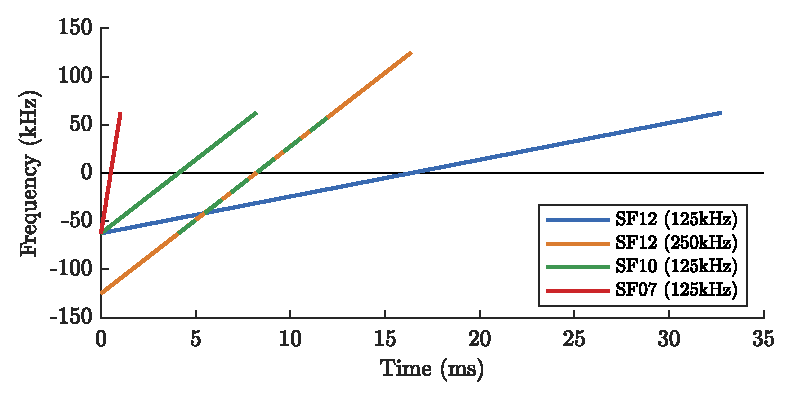
\includegraphics{Figures/sf_orthogonality_plot.eps}
    \caption[Signal chirp rate orthogonality]{
    Demonstration of signal orthogonality for different \ac{sf}s. The SF10 (125kHz) chirp is duplicated and shifted to overlap with the  SF12 (250kHz) chirp to highlight that they have the same chirp rate and are therefore not orthogonal.
    }
    \label{fig:orthogonality}
\end{figure}
%Symbol duration is the inverse of the symbol rate, defined in \ref{cr_effect}


%\section{\ac{lorawan}}\label{sec:lorawanADR}
\ac{lorawan} is a MAC layer protocol designed to be the de facto choice for point-to-multipoint \ac{lora} applications. It is largely certified worldwide, open-source, and is both managed and promoted by the LoRa Alliance\footnote{Lora Alliance,  https://lora-alliance.org/}. The expectation of a star topology means the full protocol is not suited to the sparse swarm scenario, however, individual features are of interest. In principle it is implemented as Pure ALOHA (P-ALOHA) - a simple unchecked protocol where transmission occurs whenever a transmitter has data available to send. Figure \ref{fig:lorawan_duty_cycles} explains how duty cycle limits are enforced. The unchecked approach reduces theoretical channel usage to just 18\% \cite{3YP:LORAWAN_SLOTTED}. \ac{lorawan} abstracts \ac{sf}s and \ac{bw}s into a set of orthogonal data-rates where lower data-rates have higher range \cite{3YP:LORAWAN_REGIONAL_PARAMS}; these are used by the \ac{adr} functionality mentioned in Section \ref{sec:parameter_selection}.

\begin{figure}[H]
    \centering
   	\includegraphics{Figures/duty_cycle_lorawan.pdf}
    \caption[\ac{lorawan} duty cycle enforcement]{
    Demonstration of how \ac{lorawan} enforces duty cycle limits; that is after a transmission of airtime $T_a$, the transmitter must be silent for a minimum period of $T_s=T_a(\frac{1}{d_c}-1)$ \cite{3YP:LIMITS_OF_LORAWAN}. The figure is to scale for $d_c=10\%$.
    
    }
    \label{fig:lorawan_duty_cycles}
\end{figure}


% ADR
% Operation is scheduled by a node setting the reserved \ac{adr} bit in uplink messages. The gateway responds with initial transmission parameters to attempt. The node sets its transmission parameters to these values and proceeds with the expectation that the gateway is reachable. However, if the gateway does not acknowledge any packets within a set period, the \ac{adr} bit is set again to force an acknowledgement. Failure to receive any acknowledgement implies that the gateway is not within range. Data-rate is reduced or \ac{tp} is increased until an acknowledgement is made, these are the parameters used unless a further \ac{adr} request is made. 



\section{\ac{ism} Band Regulation}\label{sec:ISMBandRegulation}
The industrial, scientific and medical (\ac{ism}) bands are portions of the radio spectrum, which can be used without a license, subject to local regulatory standards. These standards vary around the world but often define maximum power outputs, duty cycles, and bandwidths. Though limits can be problematic, they help reduce the chance of internal and external system interference. Some of the most stringent regulations are in Europe, where they are controlled firstly by the European Telecommunications Standards Institute (the \ac{etsi}\footnote{ETSI, EU, https://www.etsi.org}), and then by country specific authorities. The United States' regulations are managed by the Federal Communications Commission (the \ac{fcc}\footnote{FCC, US, https://www.fcc.gov}), with many other countries following their example. 

Sub-1GHz \ac{lora} hardware operates around the 433MHz and 900MHz bands, but as the former is very heavily regulated for non-remote controls in the US \cite{3YP:FCC_433}, only the 900MHz area is considered viable to the use case. It should be noted however that the specific frequencies used will still differ between region, as is demonstrated by \ac{lorawan}'s use of the 863-870 MHz and 902-928 MHz bands for Europe and the US respectively \cite{3YP:LORAWAN_REGIONAL_PARAMS}. A comparison of the regulations can be seen in Table \ref{tab:ISMRegions}. As \ac{etsi} limits vary heavily on a by band basis, they are broken down further in Table \ref{tab:ETSIBands}. An overview of each regulation type follows.
 
 \begin{table}[H]
\centering\small
\caption[900MHz regional regulation comparison]{Regional regulation comparison for 900MHz band radio \cite{3YP:FCC_900, 3YP:ETSI_HARMONISED_REG}.}
\label{tab:ISMRegions}
\renewcommand*{\arraystretch}{1.1}
\begin{tabular}{l|L{45mm}L{45mm}}
    \toprule
    & \textbf{\ac{fcc}} & \textbf{\ac{etsi}}  \\
    \midrule\addlinespace
    \textbf{Band} & 902--928MHz & 863--870MHz \\
    \textbf{\ac{eirp}} & {36dBm \newline \textit{  30dBm transmit power}} & {0.25MHz @ 27dBm \newline 6.40MHz @ $\leq$ 14dBm} \\
    \textbf{Duty Cycle} & None & 0.1\%--10\% \\
    \textbf{Bandwidth} & 26 MHz & 6.65MHz \\
    \textbf{Narrowband} & 400ms airtime per transmit & None\\
    \textbf{\ac{css}} & None & Varies  \\
    \addlinespace\bottomrule
\end{tabular}
\end{table}

Duty cycle limits greatly reduce the amount of airtime a radio is allowed. For example, in Band h1.3, there is a 1\% duty cycle, which indicates a maximum of 36 seconds of airtime, over all the band's channels, over a rolling one hour period. Duty cycles are considered within a band so a multi-band implementation may obey multiple duty cycles separately. Alternatively, the polite spectrum access (\ac{psa}) policy can be used; this is a defined regulation for listen before talk (LBT) implementations \ac{psa} allows airtime of up to 100 seconds per 200kHz of spectrum, per hour, regardless of duty cycle \cite{3YP:ETSI_PSA}. It does however require a clear channel assessment to be carried out before every transmission, this would be independent of \ac{lora}'s \ac{cad}.
 
\begin{table}
\centering\small
\caption[\ac{etsi} 868MHz sub-band breakdown]{\ac{etsi} 868MHz sub-bands for short range devices (adapted from \cite{3YP:ETSI_HARMONISED_REG}). Only bands relevant for \ac{css} are included. Band numbers correspond to CEPT-ERC-REC 70-03 definitions \cite{3YP:CEPT_ERC_REC}}
\label{tab:ETSIBands}
\renewcommand*{\arraystretch}{1.1}
\begin{tabular}{c|ccccc}
    \toprule
    \textbf{Band} & \textbf{Frequency} (MHz) & \textbf{\ac{eirp}} (dBm)  & \textbf{Duty Cycle} & \textbf{Max \ac{bw}} (kHz) \\
    \midrule\addlinespace
    \textbf{h1.2} & 863.00--870.00 & 14 & 0.1\% (or PSA) & 7000 \\
    \textbf{h1.3} & 865.00--868.00 & 14 & 1\% (or PSA) & 300 \\
    \textbf{h1.4} & 868.00--868.60 & 14 & 1\% (or PSA) & 600 \\
    \textbf{h1.5} & 868.70--869.20 & 14 & 0.1\% (or PSA) & 500 \\
    \textbf{h1.6} & 869.40--869.65 & 27 & 10\% (or PSA) & 250 \\
    \textbf{h1.7a} & 869.70--870.00 & 7 & None & 300 \\
    \textbf{h1.7b} & 869.70--870.00 & 14 & 1\% (or PSA) & 300 \\   
    \addlinespace\bottomrule
\end{tabular}
\end{table}

Regulations consider power as equivalent isotropically radiated power (\ac{eirp}). This value is directly related to radio transmission power ($P_t$) and can be calculated as $EIRP = P_t - L + G$ where $L$ is cable loss and $G$ is antenna gain. The latter occurring from transmit power being concentrated into a smaller area, all antenna will have some form of gain as isotropic antennas are only hypothetical. For example, a radio operating in Band h1.3, using a typical omnidirectional antenna that has 3dBi of gain, can only transmit at 11dBm if no cable loss occurs. Realistically, some cable loss will occur but this must be considered on an implementation by implementation basis. Directional antenna compound these issues due to their high-gains and the relatively low \ac{eirp} limits.

The \ac{etsi} regulations are the limiting factor in transmit power, duty cycle and overall available bandwidth. \ac{lora} being a \ac{css} signal means \ac{fcc} narrowband limitations need not be a concern. Under this consideration, the \ac{etsi} regulations will be used as the worst-fit scenario from here on in. When considering national regulation, it is common that either all bands are implemented, or none at all \cite{3YP:CEPT_ERC_REC}. Of the ETSI bands, h1.3, h1.4 and h1.6 are of most interest. h1.3 and h1.4 giving a balanced offering of bandwidth, \ac{eirp} and duty cycle. Whilst h1.6 offers a far greater duty cycle and \ac{eirp} but limited bandwidth; a further regulatory limit means only allows a single wide-band channel can operate within this band. The maximum number of possible \ac{lora} channels in each of these bands can be seen in Table \ref{tab:ETSILoraChannels}.

\begin{table}[H]
\centering\small
\caption[Maximum channel breakdown for \ac{lora}]{Maximum channel count breakdown for relevant \ac{etsi} bands, calculated for \ac{lora}'s most common operating bandwidths. Calculated assuming channel spacing is 120\%  of the bandwidth to avoid inter-channel interference.}
\label{tab:ETSILoraChannels}
\renewcommand*{\arraystretch}{1.1}
\begin{tabular}{c|ccc}
    \toprule
    & \multicolumn{3}{c}{\textbf{Channel \ac{bw}}}	\\
    \textbf{Band} & \textbf{125kHz} & \textbf{250kHz} & \textbf{500kHz}\\
    \midrule\addlinespace
    \textbf{h1.3} & 19 & 8 & N/A \\
    \textbf{h1.4} & 4 & 2 & 1 \\
    \textbf{h1.6} & 1 & 1 & 0 \\
    \addlinespace\bottomrule
\end{tabular}
\end{table}

\section{Ad-Hoc Networks}\label{sec:adhocnetworks}
\subsection{Routing}
An ad-hoc network is a type of wireless network that does not rely on any managed infrastructure, such as hard-wired routers. The network's nodes are responsible for determining their own routing paths and forwarding other nodes packets (i.e. acting as the routers). As explored by \cite{3YP:LORAWAN_MESH}, a single network could make use of multiple transmission mediums to reach the destination node. A \ac{manet} is a special type of ad-hoc network where nodes are expected to move, resulting in frequent changes to the network topology \cite{3YP:MANET_RFC2501}. If a network is sparse or operating at the limits of the transmission medium, and packet delivery is not time critical, the network can be treated as a delay-tolerant-network (\ac{dtn}). A common approach to \ac{dtn}s is to adopt store-carry-forward (\ac{scf}) behaviour; this is where intermediate nodes will keep hold of data until either a new path appears or signal strength improves \cite{3YP:DTNS}.
 
 Route management is the most researched challenge when it comes to ad-hoc networks \cite{3YP:MANET_RESEARCH_TRENDS} with implementations typically falling into the proactive or reactive categories - though more scenario specific variations do exist (e.g. geographic). Nodes using a proactive approach maintain a routing table for the whole network, to achieve this they rely on periodic updates from other nodes with their routing tables; these methods have low transmission delay but high ongoing overhead and adapt slowly to network changes. Nodes using a reactive approach explore the network when necessary to find a path, often by flooding route request packets; these methods have high transmission delay, but no ongoing overhead and can adapt to network changes immediately. Routing is not considered further in this paper so this is the abstracted level to which algorithms are considered. Full descriptions of many examples, including \ac{aodv} (reactive), \ac{olsr} (proactive) and \ac{lar} (geographic) can be found in \cite{3YP:ROUTING_ALGORITHMS}.
 

\subsection{\ac{mac} Protocols}
\label{sec:mac_protocol_background}
An ad-hoc network contains many transmitters, therefore a medium access control (\ac{mac}) protocol is required to regulate access to the shared transmission medium. The selected method has a considerable effect on network efficiency and reliability in terms of power usage, collision occurrence, throughput, latency and fairness. Protocols can be classed as either contention-free or contention-based. The former use transmission schedules; these can waste resources if nodes do not require equal channel access, and struggle to adapt to changing topologies, but can be completely collision-free. The latter rely on nodes competing for access, these are flexible as they can adapt to different topologies with little overhead, however they are not collision free. For critical communications it must be possible to detect these collisions and recover from them. This can be very costly, requiring acknowledgements and retransmissions \cite{3YP:WSN_BOOK}.

IEEE 802.11 (Wi-Fi) uses a combination of carrier-sense multiple access (\ac{csma}) and multiple access with collision avoidance (\ac{macaw}). This is where a node first senses the medium for activity, before reserving the channel by transmitting request to send (RTS) and clear to send (CTS) control messages \cite{3YP:NETWORK_BOOK}. Theoretically this will alert other nodes so they do not transmit for this duration. Although the overhead introduced is not ideal, it is acceptable for high data-rate communications and large transmissions. The reservation phase is inefficient for \ac{lora} due to its long airtimes, however, pure carrier sensing implementations using \ac{lora}'s \ac{cad} have been shown to be effective in the presence of receivable transmissions \cite{3YP:LORA_CSMA}. 

\ac{lorawan} is a \ac{mac} protocol designed to be the de facto choice for point-to-multipoint \ac{lora} applications. It is largely certified worldwide, open-source, and is both managed and promoted by the LoRa Alliance\footnote{Lora Alliance,  https://lora-alliance.org/}. The expectation of a star topology means the full protocol is not suited to the ad-hoc scenario, however, individual features are of interest. In principle it is implemented as P-ALOHA, a simple unchecked protocol where transmission occurs whenever a transmitter has data available to send. Duty cycle limits play a large part in keeping collisions at a minimum, Figure \ref{fig:lorawan_duty_cycles} explains how these are enforced. The unchecked approach reduces theoretical channel usage to just 18\% \cite{3YP:LORAWAN_SLOTTED}.

\begin{figure}[H]
    \centering
   	\includegraphics{Figures/duty_cycle_lorawan.pdf}
    \caption[\ac{lorawan} duty cycle enforcement]{
    Demonstration of how \ac{lorawan} enforces duty cycle limits; that is after a transmission of airtime $T_a$, the transmitter must be silent for a minimum period of $T_s=T_a(\frac{1}{d_c}-1)$ \cite{3YP:LIMITS_OF_LORAWAN}. The figure is to scale for $d_c=10\%$.
    }
    \label{fig:lorawan_duty_cycles}
\end{figure}
\chapter{\ac{lora} \ac{phy} Testing}

It has been repeatedly shown that \ac{lora} transmissions can be received at distances exceeding 10km in  unobstructed environments (free-space) when antennas are highly elevated \cite{3YP:LORA_RANGE_REVIEW}. However, these ideal radio conditions are unrealistic for swarm robots operating close to the ground in high-propagation environments such as forests. Therefore the first experiment in this paper identifies \ac{lora}'s physical performance and scenario specific limitations. Due to expected sparsity, only far field scenarios are relevant ($d_{\text{SP}\leftrightarrow \text{MP}} >  0.35$m).


\section{Methodology}
The purpose of this testing was to inform protocol decisions and assess capability of an off-the-shelf \ac{lora} \ac{phy}. A focus was taken to get enough data across a small selection of important scenarios and parameters to allow quantitively assessment. 

 The two main transmission environments selected were free-space and in-forest; this was to give an understanding of both low-propagation and high-propagation scenarios. Data collection was mainly spread over two locations: \textbf{$L_{A}$} and \textbf{$L_{B}$} (split into \textbf{$L_{B1}$} and \textbf{$L_{B2}$}), identified in Figure \ref{fig:new_forest_map} and \ref{fig:stansted_map} respectively. All locations were rural and therefore theoretically free from strong sources of external interference. Radio placement was decided by first placing the transmitting radio (slave) at a fixed location (\ac{sp}), and then, using the furthest receivable point as the starting point for the receiving radio (master). From there the master was positioned closer towards the slave for each future test (\ac{mp}). In each scenario the main interest was ground level transmissions; however, to assess whether radio performance was actually compromised by the placement, comparative measurements were taken with an elevated antenna. 
 
  \begin{figure}[H]
    \centering
    \includegraphics[width=\textwidth]{Figures/new_forest_light}
    \caption[Test Location: The New Forest, Hampshire, UK]{
    Test positions for \textbf{$L_A$} :  The New Forest, Hampshire, UK.\protect\footnotemark[1] \\
    \ac{sp} in open with \ac{los} to other points a combination of free-space and light vegetation. Exact positions are in Appendix \ref{sec:new_forest_test_pos}. To the left of \ac{mp}7 vegetation density increases,  making \ac{mp}7 the furthest position viable for free-space testing.
    }
    \label{fig:new_forest_map}
\end{figure}

\begingroup
 \begin{figure}[H]
    \centering
    \begin{tabular}{c}
    \subfloat[{
    Test positions for in-forest testing (\textbf{$L_{B1}$}). \ac{sp} in forest with \ac{los} to other points continually obstructed by a combination of leaved and bare trees. Exact positions are in Appendix \ref{sec:stansted_forest_test_pos}. Large clump of \ac{mp}s where radio reception was inconsistent.
    }]
    {\includegraphics[width=\textwidth]{Figures/stansted_forest}\label{fig:stansted_map_forest}} 
    \\
    \subfloat[{
        Test positions for free-space testing (\textbf{$L_{B2}$}). \ac{sp} in open with \ac{los} completely free-space. Exact positions are in Appendix \ref{sec:stansted_free_test_pos}. No access to right of \ac{mp}13.
    }]{\includegraphics[width=\textwidth]{Figures/stansted_free_space}\label{fig:stansted_map_free}}
    \end{tabular}
    \caption[Test Location: Stansted Forest, West Sussex, UK]{
    Test locations for \textbf{$L_B$} :  Stansted Forest, West Sussex, UK.\footnotemark[1]
    }
    \label{fig:stansted_map}
\end{figure}
\footnotetext[1]{
    	$\enskip $ Copyright © 2019 MapOSMatic/OCitySMap developers\\
    	\indent \indent $\enskip $ Map Data © 2019 OpenStreetMap contributors (see http://osm.org/copyright)\\
    	\indent \indent $\enskip $ British Style © MapQuest \\
    	\indent \indent $\enskip $ Contour Overlay © OpenSnowMap.org
}

 In terms of radio parameters, \ac{sf} was the main focus due to it being an on option mostly unique to \ac{lora}; all values were tested for this in all locations ($\text{\ac{sf}} = 7, 8, 9, 10$). Variations using the lowest (4/5) and highest (4/8) \ac{cr}s were collected to verify \ac{fec} performance. Additionally, as the maximum transmission unit is often defined by the protocol, the effects of varying packet length were taken (\ac{pl} = 20, 128, 255 [\ac{phy} limit]). The rest of the parameters were fixed. The 868.1MHz \ac{cf} was used with \ac{tp} set to 14dBm so that collected data would be relevant in regard to \ac{etsi} regulations. The bandwidth was fixed to 125kHz so that radio sensitivity was only affected by the \ac{sf}. The \ac{ps}s were set to 8 to match \ac{lorawan} \cite{3YP:LORAWAN_REGIONAL_PARAMS}. The number of packets (\ac{pc}) transmitted for each configuration was set to 50; though not guaranteed, this gave reasonable expectation of a normal distribution. See Table \ref{tab:TestDefinitions} for full test definitions.
 
 To test the point-to-point transmissions, two identical platforms, which together could log the performance of sending and receiving \ac{lora} transmissions, were required. The platforms had to be suitable for outdoor use, be able to test multiple radio configurations whilst on location and provide a mechanism to indicate to user when the maximum range had been reached. The hardware and corresponding software created for this purpose is detailed in Appendix \ref{sec:testing_platform}.
\begin{figure}[H]
    \centering
    \begin{tabular}{ccc}
    \subfloat[][$L_{A}$ : MP05 \\ (1.0m)]{\includegraphics[height=7.5cm]{Figures/la_MP5_H1_0}}
    \hspace{2.5mm}
    \subfloat[][$L_{B1}$ : SP \\ (0.5m)]{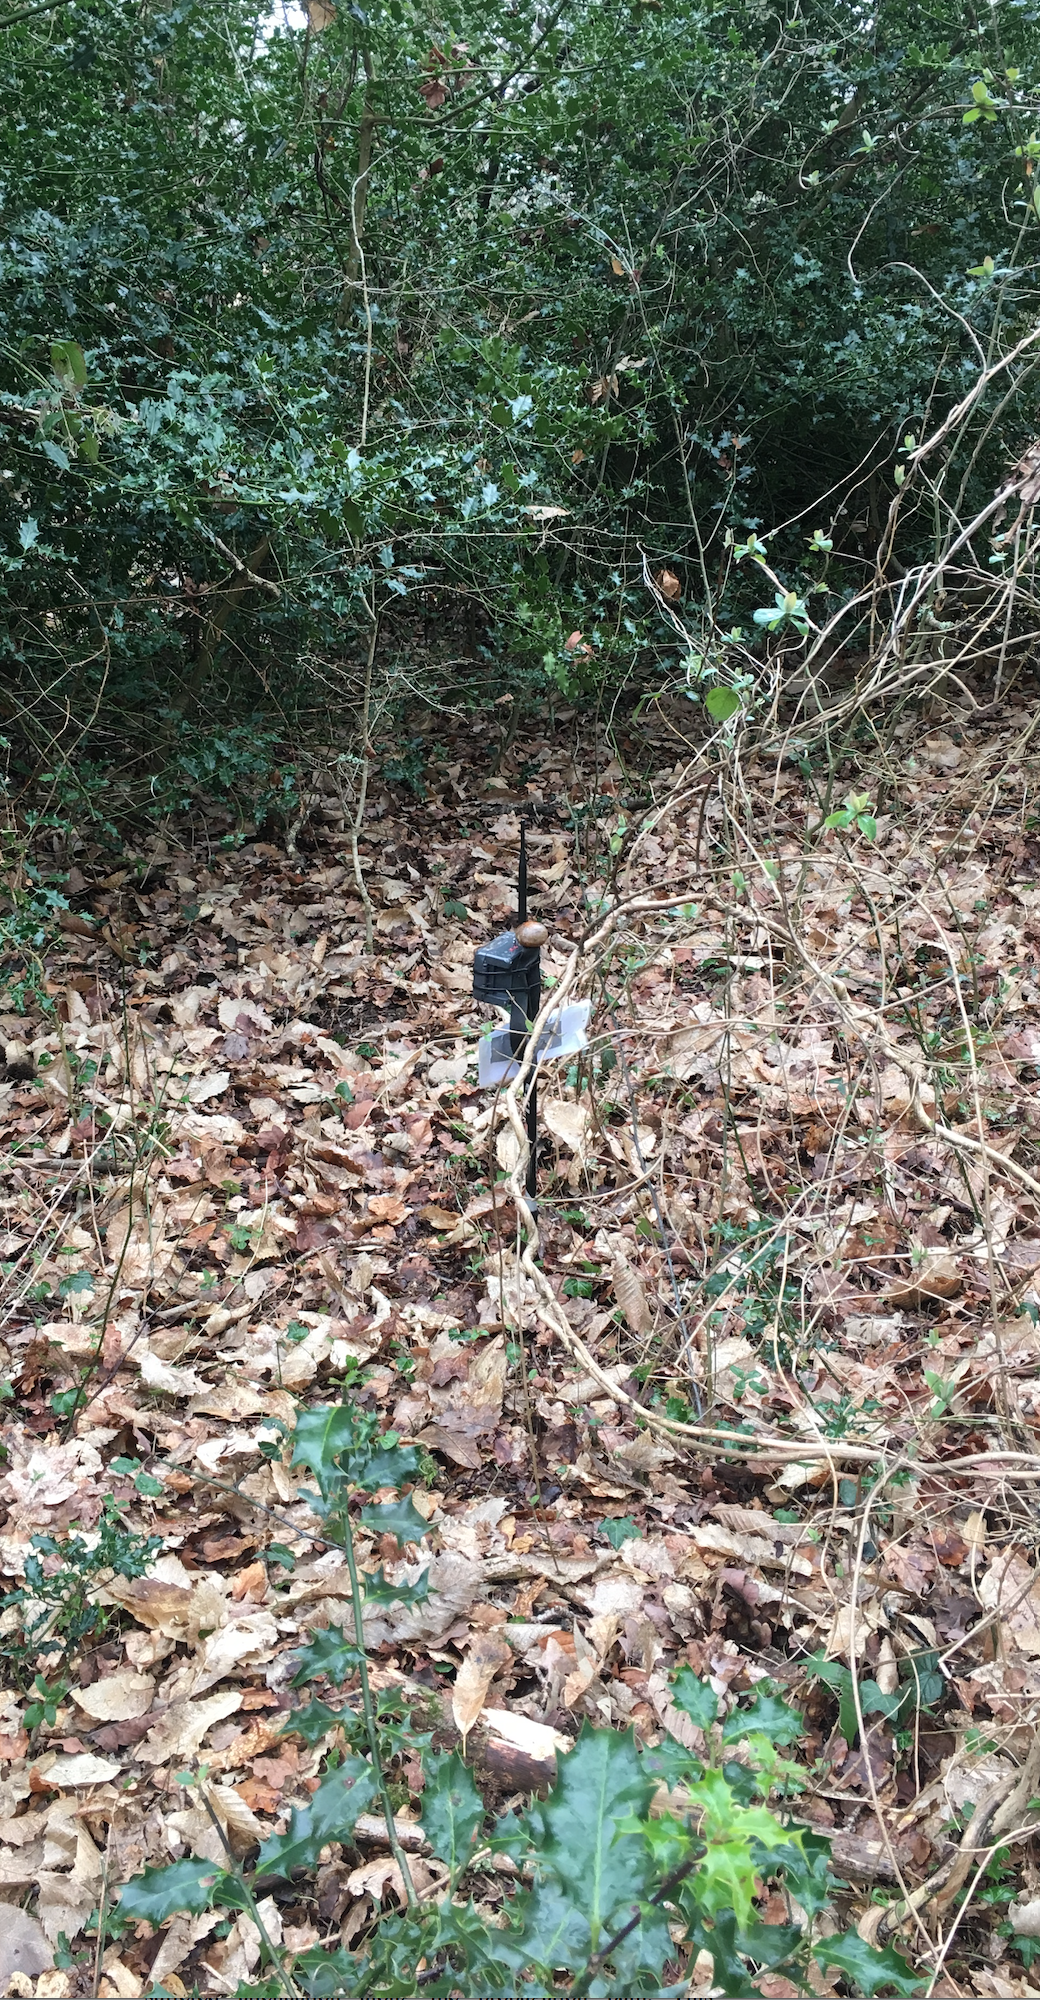
\includegraphics[height=7.5cm]{Figures/lb1_SP_H0_5}}
    \hspace{2.5mm}
    \subfloat[][$L_{B2}$ : MP16 \\ (0.0m)]{\includegraphics[height=7.5cm]{Figures/lb2_MP16_H0_0}}
    \end{tabular}
    \caption[Test location example]{Pictures of test environments and conditions. Although testing was split across multiple days at each location, the same dry conditions were present.}
    \label{fig:dataloggers}
\end{figure}
\endgroup
\vspace*{\fill}


 
\newpage
\section{Test Platform}
\subsection{Hardware}
To test point-to-point transmissions, two identical platforms that could send and receive \ac{lora} transmissions were required. The basis of the designed test platform was HopeRF's\footnote{HopeRF Microelectronics Co. Ltd, China, https://www.hoperf.com/} RFM95W - a packet radio containing a \ac{lora} transceiver design licensed from Semtech; specifically, Adafruit's\footnote{Adafruit, USA, https://www.adafruit.com/} broken out version was used. As a raw packet radio, unlike the popular Microchip RN2483, it provided direct access to the radio interface. An omni-directional 3dBi 868MHz whip antenna was connected to the radio using a soldered uFL connector and a SMA to uFL connector. It was controlled by a Teensy\footnote{Teensy, https://www.pjrc.com/teensy/} 3.6 micro-controller, which also handled all logging responsibilities. A simple breakout circuit was designed and implemented on strip-board to connect the components in a condensed package. Each breakout board featured: a JST-PH2 battery connector, a coin cell holder for the Teensy's real-time-clock (\ac{rtc}), a power switch, a two-mode software switch, and three status LEDs. The schematic can be viewed in Figure \ref{fig:datalogger_schematic}. This was packaged to fit in an IP67 rated container with an internal 1800mAh \ac{lipo} battery. Switches and SMA antenna connectors were external; these were IP67 rated and extra sealing has been added where appropriate. The final dataloggers can be seen in Figure \ref{fig:dataloggers}. The Teensy is equipped with an SD card for storage but, due to cost considerations, a GPS module could not be implemented. The full breakdown of materials can be seen in Figure \ref{fig:datalogger_cost}.

\subsection{Software}
The system was designed such that one device (a slave) could be left unattended at a fixed location and controlled by a second device (a master); this was achieved using a command control system, as seen in Figure \ref{fig:software_cmd_system}. Two command classes were defined for testing purposes; these are as follows:
\begin{itemize}
	\item {\textbf{\texttt{HB\_CMD}}} : Command to trigger simple heartbeat functionality. When a slave receives this command it sends a heartbeat response (a short packet) on the base operating configuration. If in range, the master device will pick this up and alert the user.
	\item {\textbf{\texttt{TD\_CMD}}} : Command to trigger execution of a test definition (\ac{td}). In principle, the master device requests a set of packets to be sent by the slaves using the \ac{td} configuration; this is the basis of all test functionality. The full control flow is explained in detail in Figure \ref{fig:software_testdef_execution}.
\end{itemize}

%Whether a device was a master or a slave was determined by the board identifier stored in the Teensy EEPROM; this meant the same software could be flashed onto both, reducing the chance of software version inconsistencies.

\begin{figure}[H]
    \centering
    \includegraphics{Figures/software_cmd_system.pdf}
    \caption[Master-Slave command control method]{Diagram showing Master-Slave command control method.}
    \label{fig:software_cmd_system}
\end{figure}

\begin{figure}[H]
    \centering
    \includegraphics{Figures/software_testdef_execution.pdf}
    \caption[Master-Slave test definition execution method]{Diagram showing test definition execution.}
    \label{fig:software_testdef_execution}
\end{figure}




% the user, could trigger a command to be sent from the master to the receiver. 
%
%Whether a device was a master or a slave was determined by the board identifier stored in the Teensy EEPROM; this meant the same software could be flashed onto both, reducing the chance of software version inconsistencies.
%
% 
%Interfacing with the radio was handled by the RH\_RF95 driver from the Radiohead\footnote{Radiohead, https://www.airspayce.com/mikem/arduino/RadioHead/} library; this meant that only the control logic needed to be implemented. 
%
%
% A high-level overview of the planned test method is visualised in Figure \ref{master_slave_sequence}. \label{datalogger_software}
%
%
%    
%    Initial link testing will make use of two node classes: masters and slaves. The slaves are responsible for sending packets in the configuration requested by the master device. These are in the form of test definitions (TDs) that are stored on the master's memory card and will be processed one at a time. As the proposed system utilises only nodes, slave and master must have the same \ac{sf} and \ac{bw} for receiving the TD. This base state will be hard-coded such that the expected range exceeds or matches that of the longest range TD. The master will expect a certain number of packets (PC) from the slave, those received will have performance figures such as \ac{rssi}, \ac{snr} and \ac{per} recorded to the memory card under the specific test. The slave will wait for a new test definition once the PC has been sent. The master will proceed onto the next TD once the expected test length has expired.
\section{Results}
In total 498 test cases were executed, totalling 24,900 packet transmissions. Of this total 19,545 were successfully received (78.5\%). The distribution of receive conditions for these individual points is indicated by Figure \ref{fig:density_plot}. Note that the raw \ac{rssi} values returned by the Radiohead library, and therefore the datalogger, are in fact packet strength for the SX1276 module; therefore a post-processing step has been applied to get separate packet strength and \ac{rssi} values valid for the RFM95W module. For each test definition executed, the log-mean and log-standard deviations of the successfully received packet's: \ac{rssi}, \ac{snr}, and strength have been calculated.
\begin{figure}[H]
    \centering
   	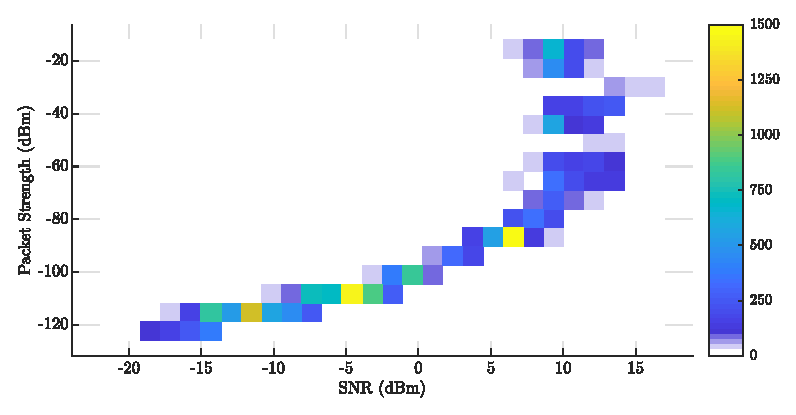
\includegraphics{Figures/density_plot}
    \caption[Test data distribution plot]{
    Density plot of received packet transmissions modelled as a bi-variate histogram with colour indicating received packet count. \\$Total\enskip Points = 19,545$
    }
    \label{fig:density_plot}
\end{figure}

\section{Discussion}
Some writing
\subsection{PHY Layer Performance}

\subsubsection{Spreading Factor}

\subsubsection{Coding Rate}

\subsubsection{Packet Length}

\begin{figure}[H]
    \centering
   	\includegraphics{Figures/snr_pp_separate_plot}
    \caption[Plots of \ac{snr} vs Packet Receive Percentage]{
   \ac{td} mean \ac{snr} values plotted against their packet receive percentages, separated by \ac{sf}s (Order = [[7, 8, 9], [10, 11, 12]]). For each \ac{sf} plot: the theoretical demodulation limit is indicated by the dotted line and the solid line corresponds to the best-fit sigmoid function; these are repeated in Figure \ref{fig:sf_pp_fit}. Although the best-fit sigmoids give a good representation of the general data pattern, and provide empirical demodulation cut-offs, they do not capture the high-variance receive behaviour when approaching the cut-off. This is reflected by the fact that only 62\%, 60\%, 66\%, 39\%, 77\% and 82\% of the respective training points fall inside the corresponding 95\% confidence interval. Notably \ac{sf}10 has very high-variance; this is reflected in the 95\% maximum receive chance. 
    }
    \label{fig:snr_pp_separate}
\end{figure}

\begin{figure}[H]
    \centering
   	\includegraphics{Figures/sf_fit_plot}
    \caption[Plot of sigmoid best-fits for \ac{snr} vs Packet Receive Percentage]{
    Plot of sigmoid best-fits generated in Figure \ref{fig:snr_pp_separate}. The plot clearly demonstrates the positive effect increasing \ac{sf} has on demodulation performance of the receiver. For \ac{sf}=7,8,9,10 demodulation success starts dropping approximately 2.5dBm before the theoretical limit ($D_L$), with a 50\% packet receive chance at $D_L$. This holds less so for \ac{sf}=11, for which drop-off starts around $D_L - 5dBm$, until $D_L$ where there is only a 10\% receive success. For \ac{sf}=12 drop-off starts around $D_L - 7.5dBm$, until $D_L$ where there is a 0\% receive success. Given that \ac{rssi} was relatively stable when $\ac{snr} < 0$, and that expected performance holds until a certain \ac{snr}, there is an indication that the sensitivity of the receiver is not as high as stated. 
     }
    \label{fig:sf_pp_fit}
\end{figure}

\subsection{Environmental Effects}
\subsubsection{Open (Free) Space}
High noise floor indicates that either the receiver's noise figure is not correct or there is more noise than expected in the environment. The fact that demodulation limit is nowhere near the true limit for SF10 onwards suggests that the cheaper radio does not perform correctly.
\subsubsection{Forest}
\subsubsection{Radio Height}
Increasing radio height massively increased range once reached 1m

% Distance in relatively open space (got)
% Distance in trees (got)
% Closeness to ground (got)
% Coding rate ??? (sort of got)
% Difference in slight movements (!!!)
%Lessons Learnt 
https://www.thethingsnetwork.org/forum/t/no-lower-rssi-than-121-dbm-possible-in-ttn/19890/15
\chapter{Simulator}
\section{Model}
\subsection{Airtime}
\label{sec:LoRaTiming}
A \ac{lora} transmission consists of a number of symbols, 
Configuration of these parameters effect transmission time
The time a \ac{lora} symbol takes to transmit can be calculated



% Time model realtime using predicted lora airtimes
% Model discrete events
\subsection{Propagation}
\subsection{RSSI}
\subsection{SNR}
\subsection{Interference}
\label{sec:RadioCollisions}

% Seperate model for collisions from 91197515.pdf
% receivers are able to detect when a collision has occurred increasing liklihood of getting second packet, this has not been implemented as its performance has not been verifiable
\subsection{Receive Chance}
% Sigmoid packet chance functions?
\subsubsection{Channel Activity Detection (CAD)}
\section{Interface (GUI)}

\chapter{MAC Protocols}\label{sec:protocols}
In this section three contention-based \ac{mac} protocols are considered to handle the requirement of data transfers to physically close neighbours: a base case (ALOHA), a common approach (\ac{csma}) and a scenario specific approach (\ac{llbp}). 

\section{Considerations}\label{sec:mac_considerations}
Designing approaches so that as many radios as possible receive a transmission is of little help; from the receiver's perspective, if local-interest data is received 1500m away, the transmission is unwanted and increasing the chance of a local collision. To this end a criteria is defined as the maximum distance for which data is `wanted'; this is set to the worst-case transmission distance (500m).

The \ac{lora} configurations used are the abstracted \ac{dr}s from \ac{lorawan} \cite{3YP:LORAWAN_REGIONAL_PARAMS}; however, DR0 and DR2 are disregarded due to their lack of respective \ac{sf} performance. Although small packets ($< 20\enskip \text{bytes}$) have been shown to have slightly higher receive probability, they are not practical with transmission overhead, therefore packets are allowed to be any size ($\leq 255\enskip bytes$). \ac{cr} and \ac{tp}s are assumed to be 4/5 and 14dBm respectively.

As opposed to \ac{lorawan}'s \ac{dc} manager (see Figure \ref{fig:lorawan_duty_cycles}), all protocols use a custom \ac{dc} manager proposed in Appendix \ref{sec:proposed_duty_cycle}. This is  more flexible because it considers airtime over the full enforcement interval ($d_i$), allowing multiple sequential transmissions without silence; this is a requirement for bulk transmissions or protocol handshakes.

\section{Approaches}
\subsection{ALOHA}
Uses \ac{lorawan}'s principle of sending data periodically provided the \ac{dc} limit allows. No carrier-sensing is carried out, but transmissions will be delayed if the transmitter is receiving at the scheduled time. For purposes of testing, the minimum spacing between transmissions is that enforced by \ac{lorawan}. Therefore, in the case that any backoff occurs, less than the \ac{dc}'s maximum worth of data will be transmitted. \ac{mac} performance purely relies on each radio only using a small amount of airtime. As all radios must be on the same configuration the method can only use a single channel and \ac{dr} -- no mechanism is used for dynamically agreeing parameter changes. Consequently, a fixed \ac{dc} of up to 10\% is supported on band h1.6. Test packets use random payload sizes and all packets are treated as data.

\subsection{CSMA}
Uses the ALOHA approach but does carrier-sensing using \ac{lora}'s \ac{cad} process immediately before transmissions. On detection, random backoff will occur before the \ac{cad} process repeats; this is a simplified approach to that proposed in \cite{3YP:LORA_CSMA}. The \ac{ps}s are increased from 8 to 32 to increase preamble detection likelihood with the drawback of increased airtime overhead. When all nodes are within range of one another the vulnerable collision period is very short; provided no failed synchronisations take place, collisions should only occur if two transmitter's \ac{cad}s overlap; collisions resulting from the hidden node problem (Figure \ref{fig:hidden_node_problem}) are not avoided.

\begin{figure}[H]
    \centering
   	\includegraphics{Figures/hidden_node_problem}
    \caption[Demonstration of hidden node problem]{
    	Demonstration of the hidden node problem. A has transmitted before C, however, C was unable to sense A and assumes it is okay to transmit, resulting in a collision at B \cite{3YP:WSN_BOOK}.
    }
    \label{fig:hidden_node_problem}
\end{figure}


\subsection{LoRa Local Broadcast Protocol (\ac{llbp})}
This is a bespoke approach that makes use of dynamic channel and \ac{sf} switching with the target of constricting receivability to local listeners. The protocol uses two bands: a management-band (h1.4) and a data-band (h1.3). The former is treated as a single \ac{csma} channel, whereas the latter allocates 15 channels at \ac{cf}s $865.1 + 0.2 \cdot C_n$ (\ac{bw}=125kHz).

In principle, the protocol announces when a transmitter has a large chunk of data to send using a data announcement packet (\ac{dap}); this contains the \ac{lora} configuration to switch to and a description of the data being sent (Figure \ref{fig:dap_packet}). When a radio receives this packet it can make its own decision on whether it wants the data; if it does not it can ignore the message and will never see any data packets, otherwise it can switch configurations and only see those packets. This dump behaviour is heavily suited to \ac{scf} situations.

\begin{figure}[H]
    \centering
   	\includegraphics{Figures/dap}
    \caption[Data Announcement Packet (\ac{dap})]{
 		 \ac{dap} structure. The number of data packets being sent and their average length is provided so the receiver can timeout appropriately in case no packets arrive. The delay field is provided to indicate the relative start time to allow multiple \ac{dap}s. The target can be set to make announcements unicast.
    }
    \label{fig:dap_packet}
\end{figure}

As opposed to agreeing the configuration with a flurry of transmissions at one point, the configuration is decided by the transmitter, using its prior knowledge of surrounding transmitters. This knowledge is gained through periodical heartbeat packets (Figure \ref{fig:heartbeat_packet}), sent on the management-band; these provide \ac{snr}s and locations. The fastest viable \ac{dr} is picked along with a random data-band channel. There is no guarantee the channel is free but with the number of available channels, and a compulsory 1\% \ac{dc} across all of them, collisions are unlikely. \ac{dr} is selected such that for wanting receivers $\min(\text{\ac{snr}}) > (D_L + 2.5)$; this is where \ac{prp} should be approximately 100\%. The side effect of choosing the fastest \ac{dr} is less airtime; although this could be used to achieve more throughput, instead it is used to keep interference times to a minimum for the same data.

\begin{figure}[H]
    \centering
   	\includegraphics{Figures/heartbeat_packet}
    \caption[Heartbeat Packet]{
    	Heartbeat structure. Transmits a sender's location with \ac{snr} inferred. A payload can be attached to avoid wasted overhead.	
    }
    \label{fig:heartbeat_packet}
\end{figure}


\section{Test Methodology}
Protocol testing was executed on one of the simulator environment presets, \texttt{LargeData} \texttt{BroadcastTest}. The preset provided automatic generation of an $[x \times y]$ radio grid where spacing ($S$) was the same $\pm 20\%$. It provided four obstruction options seen in Figure \ref{fig:large_broadcast_options}.

\begin{figure}[H]
    \centering
   	\includegraphics{Figures/test_environments}
    \caption[\texttt{LargeDataBroadcastTest} obstruction options]{
    	\texttt{LargeDataBroadcastTest} obstruction options, green indicates forest where $\beta = 0.55$. Radios are scattered in the black square
    }
    \label{fig:large_broadcast_options}
\end{figure}
If radios were always able to use their fastest configuration, it was unlikely a protocol with overhead would outperform one without. To alleviate this unfairness, $S$ was set to 400m; ensuring that in-forest radios needed \ac{dr}1 to communicate, but giving other transmissions the opportunity to increase \ac{dr}. 

The protocol configurations executed for each environment were:
\vspace{-5mm}
\begin{itemize}
\item ALOHA with \ac{dc}s of 1\% \textbf{[A]} and 10\% \textbf{[B]}.
\item CSMA with \ac{dc}s of 1\% \textbf{[C]} and 10\% \textbf{[D]}.
\item \ac{llbp} with \ac{dap} count of 1 \textbf{[E]} and 2 \textbf{[F]}.
\item \ac{llbp} with \ac{dap} count of 1 where true locations and \ac{snr} values were known \textbf{[G]}. This can be considered as \ac{llbp}'s best case performance but is not representative of actual performance. 
\end{itemize}
\vspace{-5mm}
For \ac{llbp} heartbeats were sent for 1/2 of the management-band airtime. 1/6th of the data-band airtime was sent after each \ac{dap}; meaning 6 \ac{dap}s an hour. Movement was not simulated but received heartbeats timed out after 10 minutes to reflect that movement is expected.

Each of the 28 configurations was executed in the simulator for 6 hours of simulation time, after which simulator statistics were exported.


\section{Results \& Discussion}
Each protocol is assessed by: its throughput of \textit{wanted} data per transmitter over the simulation period ($T$)  and the delivery percentage (DP). Together giving an understanding of the effective throughput. Aggregated results are seen in Figure \ref{tab:protocol_results} with separated box-plots of the two metrics in Figure \ref{fig:sim_throughput_boxplots} and Figure \ref{fig:sim_recv_boxplots} respectively.

\begin{table}[H]
\centering\small
\caption[Aggregated protocol testing results]{
Results aggregated by protocol, taking the mean of each transmitter across all environments. 
} 
\label{tab:protocol_results}
\renewcommand*{\arraystretch}{1.1}
\begin{tabular}{c|cc}
    \toprule
    \textbf{Configuration} & \makecell{Throughput (KB)} & DP (\%)  \\
    \midrule\addlinespace
    \textbf{A} & 35 & 91 \\
    \textbf{B} & 203 & 69 \\
    \textbf{C} & 30 & 91\\
    \textbf{D} & 183 & 77 \\
    \textbf{E} & 18 & 47 \\
    \textbf{F} & 34 & 52 \\
    \textbf{G} & 31 & 86 \\   
    \addlinespace\bottomrule
\end{tabular}
\end{table}

Unsurprisingly, throughputs are clustered by \ac{dc}, where $T_{10\%} \gg  T_{1\%}$. It could be expected that $10\times $ the \ac{dc} would result in $10\times $ the throughput; however the actual increase for both ALOHA and \ac{csma} is approximately $ 6\times$. The other $4\times $ accounted for by: backoff from the cluttered airspace ($\text{ALOHA}=1.9\times $, $\text{\ac{csma}}=2.5\times$), and more frequent failed/missed receives ($\text{ALOHA}=2.3\times $, $\text{\ac{csma}}=1.4\times$). Low DP, as a result of collisions and busy receivers, leads to unpredictability, increasing overhead caused by acknowledgements and retransmissions. The drops in DP for $\text{A}\rightarrow \text{B}$ and $\text{C}\rightarrow \text{D}$ are 22\% and 14\%. If these dropped packets require retransmissions, without considering acknowledgements, effective throughput drops to 47\% and 63\% respectively; considerations like these are implementation specific. Even given these arguments, effective throughput will usually improve by increasing \ac{dc} though more testing is required to find the limit. The 10\% drop in throughput and 8\% increase in DP for $\text{B}\rightarrow \text{D}$ indicates that \ac{csma} is only worth the overhead when taking retransmissions into account - if guaranteed receives are not required, ALOHA is more efficient.
%82 bytes 82 / 350 23.4%
%65 backoff 65 / 350 18.6\%
%42 bytes collisions 42 /300 14%
%75 backoff 75 / 300 = 25%
\vspace{10mm}
\begin{figure}[H]
    \centering
   	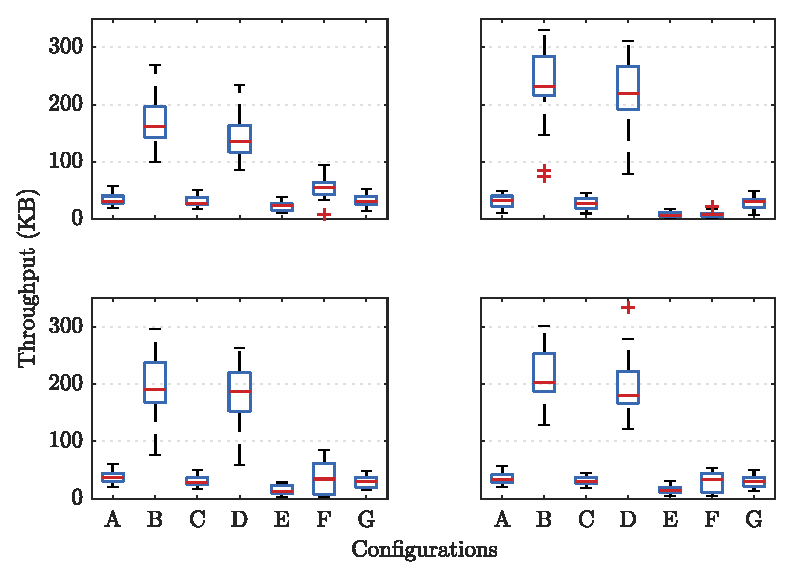
\includegraphics{Figures/sim_throughput_boxplots}
    \caption[Box-plots of protocol transmitter throughput]{
    	Box-plots of each transmitter's throughput in each environment [[A, B], [C, D]]. They demonstrate the throughput advantage of higher duty cycles and with that, higher variance between individual transmitter's access to the medium.}
    \label{fig:sim_throughput_boxplots}
\end{figure}

With this established, direct comparisons cannot be made between \ac{llbp} and configurations with 10\% \ac{dc}s. However, it is immediately clear that the \textit{fair} \ac{llbp} implementations do not out perform the 1\% ALOHA and \ac{csma} configurations; as is demonstrated by $P_{E || F} \ll P_{A||C}$ and $T_{E || F} \leq T_{A||C}$. Even with the best (\textit{cheat}) \ac{llbp} case, G has significantly less DP than the simpler approaches. Figure \ref{fig:sim_failure_reasons} indicates that the receiver can often not see data packets for \ac{llbp} configurations, indicating that the receiver does not switch bands correctly. This is likely caused by \ac{dap} receive failures; the theory made more likely by the significant increase of DP ($p = 0.01$) for $\text{E}\rightarrow \text{F}$. This issue is likely due to less critical heartbeat packets colliding with \ac{dap}s.
\newpage
 That being said, the far more significant problem can be seen by comparing E to G. G uses the same \ac{dap} count but has perfect data for \ac{dr} selection. The increase in performance indicates that transmitter decisions made by E/F are not informed by enough data, resulting in an overly aggressive \ac{dr}s being selected. These problems could be remedied by: increasing the heartbeat timeout, though this will slow down topology updates, or making heartbeats more frequent/descriptive, though this will increase \ac{dap} loss chance. To facilitate these changes the management-band could be switched to h1.6 (\ac{dr}=10\%), though this removes the possibility of having a separate high-rate channel for critical communications. 
\vspace{2cm}
\begin{figure}[H]
    \centering
   	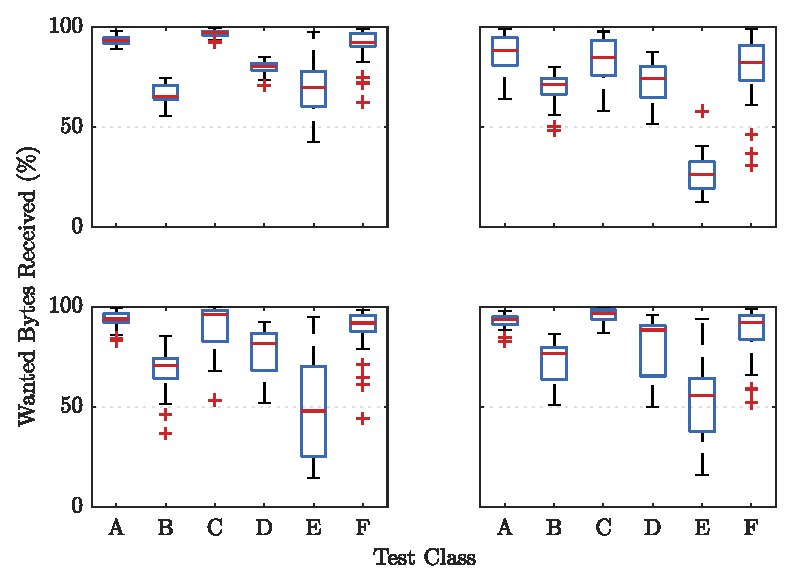
\includegraphics{Figures/sim_recv_boxplots}
    \caption[Box-plots of protocol data delivery percentage]{
    	Box-plots of DP in each environment [[A, B], [C, D]]. Highlighted is the consistency of ALOHA and \ac{csma} between environments. \ac{llbp}'s failings to select the correct \ac{dr} are highlighted by it only having acceptable performance in Environment A where any \ac{dr} will do.

    \label{fig:sim_recv_boxplots}
    }	
\end{figure}

\begin{figure}[H]
    \centering
   	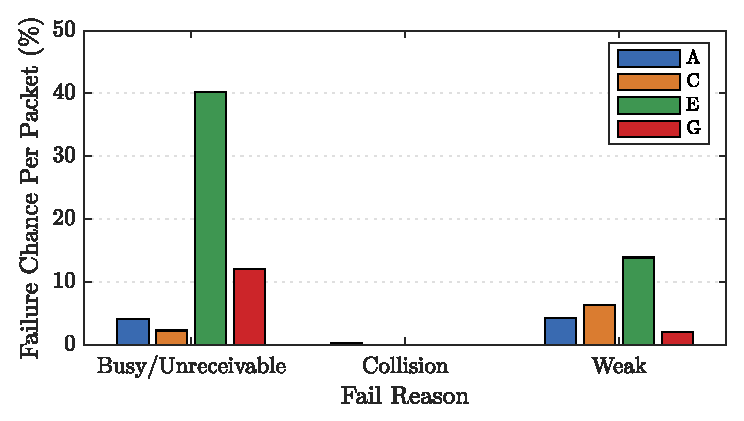
\includegraphics{Figures/sim_failure_reasons}
    \caption[Failure probabilities for protocol data packets]{
    Number of packet failures per configuration normalised by number of possible packet failures. Busy failures may have occurred due to the receiver: being synchronised with a stronger signal, doing CAD or being on the wrong configuration. Some collisions are recorded as weak due to general noise increases reducing demodulation success.
    \label{fig:sim_failure_reasons}
    }	
\end{figure}

\chapter{Conclusion}
Provided a flexible research platform both physically and simulator
Demonstrated how lora features can be taken advantage of

Future work:
Incorporation with a routing protocol
Real world testing
% Future work 
% Look at security
% Test in hardware
% Incorporate into full network stack
\chapter{Retrospective}
Ideally would have had rain data but data loggers messed up

A lot of work was put into the test platform software before changed to simulation

% 40 hours or so of on site data collection
% Lost time from trying to develop on hardware
% 


\printbibliography

\appendix
\chapter{Design Archive}
\begingroup
\raggedright\small
\definecolor{folderbg}{RGB}{124,166,198}
\definecolor{folderborder}{RGB}{110,144,169}
\newlength\Size
\setlength\Size{4pt}
\tikzset{%
  folder/.pic={%
    \filldraw [draw=folderborder, top color=folderbg!50, bottom color=folderbg] (-1.05*\Size,0.2\Size+5pt) rectangle ++(.75*\Size,-0.2\Size-5pt);
    \filldraw [draw=folderborder, top color=folderbg!50, bottom color=folderbg] (-1.15*\Size,-\Size) rectangle (1.15*\Size,\Size);
  },
  file/.pic={%
    \filldraw [draw=folderborder, top color=folderbg!5, bottom color=folderbg!10] (-\Size,.4*\Size+5pt) coordinate (a) |- (\Size,-1.2*\Size) coordinate (b) -- ++(0,1.6*\Size) coordinate (c) -- ++(-5pt,5pt) coordinate (d) -- cycle (d) |- (c) ;
  },
}
\forestset{%
  declare autowrapped toks={pic me}{},
  pic dir tree/.style={%
    for tree={%
      folder,
      font=\ttfamily,
      grow'=0,
    },
    before typesetting nodes={%
      for tree={%
        edge label+/.option={pic me},
      },
    },
  },
  pic me set/.code n args=2{%
    \forestset{%
      #1/.style={%
        inner xsep=2\Size,
        pic me={pic {#2}},
      }
    }
  },
  pic me set={directory}{folder},
  pic me set={file}{file},
}


Overview of folder structure in the design archive, not all low-level folders are indicated.\\
\vspace{5mm}

\begin{forest}
  pic dir tree,
  where level=0{}{
    directory,
  },
[design\_archive.zip, file
  [datalogger\_schematic
  ]
  [datalogger\_source
    [LoRa\_Datalogger
    ]
    [LoRa\_Board\_ID\_Setter
    ]
  ]
  [logged\_data
    [location\_pictures
  	]
  	[location\_results
  	]
  	[testdefs
  	]
  ]
  [processing\_scripts
  ]
  [simulator\_output\_data
  ]
  [simulator\_source
      [LoRa\_Simulator
    ]
  ]
]
\end{forest}

\textit{PlatformIO build files provided for datalogger source} \\
\textit{Maven POM (Project Object Model) file provided for building simulator.}

\textit{MATLAB scripts require the library functions \texttt{sigm\_fit}\footnote{\texttt{sigm\_fit.m}, rpavao@gmail.com, 2016}, \texttt{vline}/\texttt{hline}\footnote{\texttt{vline.m}/\texttt{hline.m}, Brandon Kuczenski, Kensington Labs, 2001} and \texttt{haversine}\footnote{\texttt{haversine.m}, Josiah Renfree, 2010}}
\endgroup




\chapter{Datalogger Schematic}
\begin{figure}[H]
    \centering
    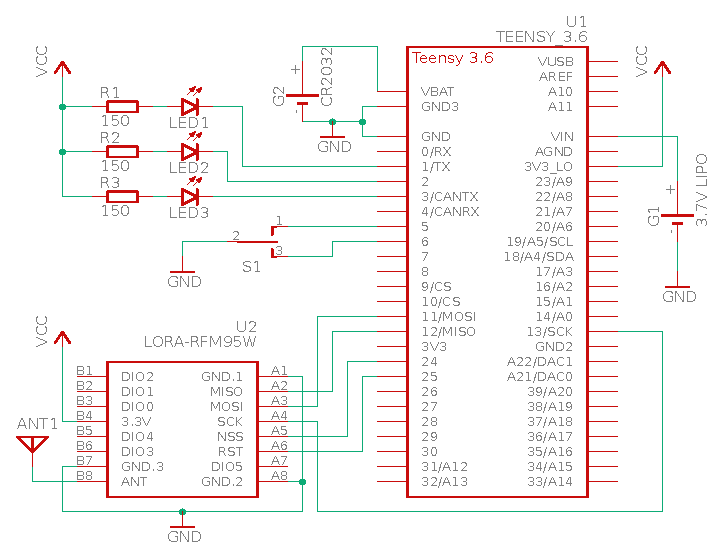
\includegraphics[width=\textwidth]{Figures/datalogger_schematic.eps}
    \caption[Schematic for datalogger hardware]{Autodesk EAGLE schematic for datalogger hardware.}
    \label{fig:datalogger_schematic}
\end{figure}

\chapter{Datalogger User Manual}\label{sec:user_manual}
\textbf{User Manual for Datalogger Software} \\ 
Firmware Version v1.0

\textbf{Overview}\\
The firmware in contained in the design archive, see \texttt{LoRa\_Datalogger}. The same firmware is used for Master and Slave devices to reduce the chance of inconsistent behaviour. The 8-bit board identifier, which is stored in Teensy EEPROM, is used to determine datalogger type. The top two bits are reserved, with B7 identifying a Master and B6 identifying a Slave, all other bits should be used to assign a unique identifier. A tool is provided in the design archive to set this appropriately, see \texttt{LoRa\_Board\_ID\_Setter}.

Full detail of master-slave commands and their purpose are included in Section \ref{sec:test_platform_software} of the main report; this manual is to instruct on how the software actually operates.

\textbf{Hardware}\\
The following hardware positions are for a device oriented such that the Teensy is on the left, the radio is on the right and the transparent top is facing upwards.

The status LEDs are as follows: \\
\phantom{-}\hspace{1cm}Bottom - \textbf{\texttt{LED\_1}} \\
\phantom{-}\hspace{1cm}Middle - \textbf{\texttt{LED\_2}}\\
\phantom{-}\hspace{1cm}Top - \textbf{\texttt{LED\_3}}

Switches are as follows: \\
\phantom{-}\hspace{1cm}Left - \textbf{\texttt{POWER\_SWITCH}} \\
\phantom{-}\hspace{1cm}Right - \textbf{\texttt{SOFTWARE\_SWITCH}}

\newpage\textbf{Common Power-On Behaviour}\\
All device types carry out the same boot sequence before device type specific behaviour, this is as follows:
\begin{enumerate}[label=\textbf{\arabic*}]
	\item  Before powering on the device, the \textbf{\texttt{SOFTWARE\_SWITCH}} can optionally be set to its bottom position to delay boot up until a serial monitor is attached to the Teensy USB. Other positions will boot up as normal. Waiting can be cancelled during boot-up by changing the switch back to any other position.
	\item Power on device by setting the \textbf{\texttt{POWER\_SWITCH}} to its bottom position. All other positions indicate off.
	\item \textbf{\texttt{LED\_1}}, \textbf{\texttt{LED\_2}} and \textbf{\texttt{LED\_3}} will turn on.
	\item The datalogger will initialise serial communications.
	\item \textbf{\texttt{LED\_3}} will turn off.
	\item The datalogger will sync with the real time clock (\ac{rtc}).
	\item The datalogger will check if it is a master or a slave using the board identifier stored in the EEPROM. If the identifier is not found or is invalid, the device will go into error state.
	\item The radio will initialise using the hardcoded configuration. On initialisation failure the device will go into error state.
	\item \textbf{\texttt{LED\_1}} will turn off.
	\item The SD card will initialise. If this is unsuccessful, boot-up will not fail but not all functionality may be available.
	\item If the \textbf{\texttt{SOFTWARE\_SWITCH}} switch is not in its middle position then boot-up will pause until it is.
	\item \textbf{\texttt{LED\_2}} will turn off.	
\end{enumerate}

When boot up is finished either \textbf{\texttt{LED\_1}} or \textbf{\texttt{LED\_3}} will be lit continuously indicating if the board is a Slave or Master respectively. If an error state is entered then \textbf{\texttt{LED\_2}} will flash continuously. The device must be rebooted to resolve this. It is suggested that a serial connection is connected before boot to discover any issues.

\newpage\textbf{Slave Behaviour}\\
Behaviour is dictated by \texttt{SOFTWARE\_SWITCH} position:
\vspace{-5mm}
\begin{itemize}
	\item \textbf{Bottom} : No Behaviour \textit{(Reserved)}
	\item \textbf{Middle} : Idle
	\item \textbf{Top} : Command Handling Mode
\end{itemize}
All modes use \textbf{\texttt{LED\_2}} to indicate a successful send or receive, and  \textbf{\texttt{LED\_1}} to indicate any failures. Behaviour can be cancelled at any time by returning the \texttt{SOFTWARE\_SWITCH} switch to the middle position.

\textbf{Master Behaviour}\\
During boot, if any of the following folders/files do not exist, they are created:
\vspace{-5mm}
 \begin{itemize}
 \item \texttt{/testdefs/} - Folder for placing test definitions.
 \item \texttt{/results/} - Folder that results are saved to.
 \item \texttt{/testdefs/\_format.txt} - File with current firmware's expected format for test definitions. As of v1.0 this is a file containing the following fields: \texttt{exp\_range,\\packet\_cnt,packet\_len,freq,sf,tx\_dbm,bw,cr4\_denom,preamble\_syms,crc,}\\ \textit{Note that the final comma is required, examples are provided in the design archive}
 \end{itemize}


Behaviour is dictated by \texttt{SOFTWARE\_SWITCH} position:
\vspace{-5mm}
\begin{itemize}
	\item \textbf{Bottom} : Heartbeat Mode. Sends continuous heartbeat commands, \textbf{\texttt{LED\_2}} will flash for a received response, \textbf{\texttt{LED\_1}} will flash for failure.
	\item \textbf{Middle} : Idle
	\item \textbf{Top} : Test Definition Mode. If the SD card is not present then this mode will not have any behaviour. Otherwise, all test definitions will be loaded and executed in order of expected range (longest range first). If no packets are received at a range level, the remaining test definitions are not executed. A test definition's results are stored in a single file, in a folder timestamped with the time the mode was executed. \textbf{\texttt{LED\_2}} indicates a test definition is being executed. \textbf{\texttt{LED\_1}} will flash on test definition delivery failure. All LEDs will be lit when the test finishes.
\end{itemize}
Behaviour of any mode can be cancelled at any time by returning the \texttt{SOFTWARE\_SWITCH} switch to the middle position.












\chapter{Test Definitions}

\begin{table}[H]
\centering\small
\caption[Test definitions for executed tests]{List of tests where each test is repeated for each spreading factor.}
\label{tab:TestDefinitions}
\begin{tabular}{C{2.5cm}|ccccccccc}
\toprule
\textbf{\ac{td}} & \textbf{\ac{pc}} & \textbf{\ac{ps}} & \textbf{\ac{cf}} (MHz) & \textbf{\ac{sf}} & \textbf{\ac{tp}} (dBm) & \textbf{\ac{bw}} (kHz) & \textbf{\ac{cr}} & \textbf{\ac{pl}} \\
\midrule

\textbf{SF\#\_A} & \multirow{4}{*}{50} & 20 & \multirow{4}{*}{868.1} & \multirow{4}{*}{All} & \multirow{4}{*}{14} & \multirow{4}{*}{125} & 4/5 & \multirow{4}{*}{8} \\
\textbf{SF\#\_B} &  & 128 &  &  &  &  & 4/5 &  \\
\textbf{SF\#\_C} &  & 255 &  &  &  &  & 4/5 &  \\
\textbf{SF\#\_D} &  & 128 &  &  &  &  & 4/8 &  \\

\addlinespace\bottomrule
\end{tabular}
\end{table}

\begin{table}[H]
\centering\small
\caption[Reference of tests executed at test locations]{Reference of tests executed at test locations. A single column refers to all spreading factors for the corresponding test. Green indicates that test was executed for all \ac{mp}s, yellow indicates that it was executed for some \ac{mp}s red indicates that the tests were not executed.}
\label{tab:LocationTestReference}
\begin{tabular}{C{2.5cm}|c|C{2cm}C{2cm}C{2cm}C{2cm}}
\toprule
\textbf{Location} & \textbf{$A_h$} & \textbf{SF\#\_A} & \textbf{SF\#\_B} & \textbf{SF\#\_C} & \textbf{SF\#\_D}  \\
\midrule
\multirow{3}{*}{\shortstack{\textbf{$L_{A}$}\\(Free-Space)}} & 1.0 & \cellcolor{green!25}{} & \cellcolor{green!25} & \cellcolor{green!25} & \cellcolor{red!25} \\
& 0.5 & \cellcolor{red!25} & \cellcolor{red!25} & \cellcolor{red!25} & \cellcolor{red!25} \\
& 0.0 & \cellcolor{red!25} & \cellcolor{red!25} & \cellcolor{red!25} & \cellcolor{red!25} \\
\addlinespace
\multirow{3}{*}{\shortstack{\textbf{$L_{B1}$}\\(Free-Space)}} & 1.0 & \cellcolor{red!25} & \cellcolor{red!25} & \cellcolor{red!25} & \cellcolor{red!25}  \\
& 0.5 & \cellcolor{red!25} & \cellcolor{red!25} & \cellcolor{red!25} & \cellcolor{red!25} \\
& 0.0 & \cellcolor{red!25} & \cellcolor{green!25} & \cellcolor{red!25} & \cellcolor{red!25}\\
\addlinespace
\multirow{3}{*}{\shortstack{\textbf{$L_{B2}$}\\(In-Forest)}} & 1.0 & \cellcolor{yellow!25} & \cellcolor{green!25} & \cellcolor{yellow!25} & \cellcolor{yellow!25} \\
& 0.5 & \cellcolor{yellow!25} & \cellcolor{green!25} & \cellcolor{yellow!25} & \cellcolor{yellow!25}\\
& 0.0 & \cellcolor{yellow!25} & \cellcolor{green!25} & \cellcolor{yellow!25} & \cellcolor{yellow!25}\\
\addlinespace\bottomrule
\end{tabular}
\end{table}


\section{$L_A$ : The New Forest}\label{sec:new_forest_test_pos}

\begin{table}[H]
\centering
\caption[Testing positions for $L_A$]{Testing positions for $L_A$. Distances calculated from \ac{sp}, which was located at [ 50.917493, -1.650739 ]. See Figure \ref{fig:new_forest_map} for approximate map. Distances calculated using haversine formula. }
\begin{tabular}{ccc}
    \toprule
\textbf{\ac{mp}} & \textbf{[Latitude, Longitude]} (DD) & \textbf{Distance} (m)\\
    \midrule\addlinespace
1 & [ 50.914819, -1.655519 ] & 448 \\
2 & [ 50.914070, -1.657508 ] & 608 \\
3 & [ 50.912152, -1.663287 ] & 1061 \\
4 & [ 50.907922, -1.672706 ] & 1872 \\
5 & [ 50.903447, -1.675974 ] & 2360 \\
6 & [ 50.902104, -1.684418 ] & 2916 \\
7 & [ 50.892091, -1.690585 ] & 3973 \\
    \addlinespace\bottomrule
\end{tabular}
\end{table}

\section{$L_{B1}$ : Stansted Forest (Free-Space)}\label{sec:stansted_free_test_pos}

\begin{table}[H]
\centering
\caption[Testing positions for $L_{B1}$]{Testing positions for $L_{B1}$. Distances calculated from \ac{sp}, which was located at [ 50.890940, -0.949549 ]. See Figure \ref{fig:stansted_map_forest} for approximate map. Distances calculated using haversine formula.}
\begin{tabular}{ccc}
    \toprule
\textbf{\ac{mp}} & \textbf{[Latitude, Longitude]} (DD) & \textbf{Distance} (m)\\
    \midrule\addlinespace
1 & [ 50.889363, -0.937320 ] & 876 \\
2 & [ 50.890099, -0.942007 ] & 537 \\
3 & [ 50.890207, -0.946020 ] & 261 \\
4 & [ 50.890243, -0.942514 ] & 499 \\
5 & [ 50.889905, -0.943777 ] & 421 \\
6 & [ 50.890070, -0.943274 ] & 451 \\
7 & [ 50.890023, -0.942815 ] & 483 \\
8 & [ 50.890095, -0.943002 ] & 469 \\
9 & [ 50.890135, -0.942476 ] & 504 \\
10 & [ 50.889955, -0.942310 ] & 519 \\
11 & [ 50.889959, -0.942100 ] & 534 \\
12 & [ 50.890024, -0.944937 ] & 339 \\
    \addlinespace\bottomrule
\end{tabular}
\end{table}


\section{$L_{B2}$ : Stansted Forest (In-Forest)}\label{sec:stansted_forest_test_pos}

\begin{table}[H]
\centering
\caption[Testing positions for $L_{B2}$]{Testing positions for $L_{B2}$. Distances calculated from \ac{sp}, which was located at [ 50.890256, -0.952222 ]. See Figure \ref{fig:stansted_map_free} for approximate map. Distances calculated using haversine formula.}
\begin{tabular}{ccc}
    \toprule
\textbf{\ac{mp}} & \textbf{[Latitude, Longitude]} (DD) & \textbf{Distance} (m)\\
    \midrule\addlinespace
13 & [ 50.888434, -0.929254 ] & 1624 \\
14 & [ 50.888534, -0.930210 ] & 1556 \\
15 & [ 50.888711, -0.932631 ] & 1385 \\
16 & [ 50.888947, -0.934794 ] & 1231 \\
17 & [ 50.889190, -0.937282 ] & 1055 \\
18 & [ 50.889580, -0.941400 ] & 763 \\
19 & [ 50.889904, -0.945198 ] & 494 \\
20 & [ 50.890217, -0.948392 ] & 269 \\
21 & [ 50.890349, -0.950226 ] & 140 \\
22 & [ 50.890476, -0.951415 ] & 62 \\
23 & [ 50.890360, -0.951811 ] & 31 \\
    \addlinespace\bottomrule
\end{tabular}
\end{table}


% \chapter{Gantt Charts}

% Current work
\begin{figure}[H]
\centering
\begin{ganttchart}[vgrid, hgrid]{1}{14}
  \gantttitle{Week}{14} \\
  \gantttitlelist{1,...,14}{1} \\
\ganttbar{Project decision\ \ }{1}{2} \\
\ganttbar{Brief writing\ \ }{2}{2} \\
\ganttmilestone{Project Brief\ \ }{2} \\
\ganttlink{elem1}{elem2}
\ganttbar{Research\ \ }{3}{13} \\
\ganttbar{LoPy Testing\ \ }{3}{7} \\
\ganttbar{RFM95 Testing\ \ }{9}{10} \\
\ganttbar{Datalogger design\ \ }{11}{12} \\
\ganttlinkedbar{Datalogger construction\ \ }{12}{13} \\
\ganttbar{Interim report writing\ \ }{11}{13} \\
\ganttmilestone{Interim Report\ \ }{13} 
\ganttlink{elem8}{elem9}
\end{ganttchart}
\caption[Interim report Gantt chart]{Gantt chart for work up to interim report (week 13)}
\label{pastgantt}
\end{figure}
\newpage

% Planned work
\vspace*{\fill}
\begin{figure}[H]
\centering
\begin{ganttchart}[vgrid, hgrid]{1}{22}
  \gantttitle{Week}{22} \\
  \gantttitlelist{14,...,35}{1} \\
\ganttbar{Datalogger software\ \ }{1}{2} \\
\ganttlinkedbar{LoRa field testing\ \ }{2}{4}
\ganttbar{}{7}{8} \\
\ganttbar[bar/.append style={fill=red}]{Exam period\ \ }{5}{6} \\
\ganttlink{elem3}{elem2}
\ganttlinkedbar{Data analysis\ \ }{8}{10} \\
\ganttbar{Simulator development\ \ }{9}{11} \\
\ganttbar{Protocol development\ \ }{11}{17} \\
\ganttbar{Protocol analysis\ \ }{13}{17} \\
\ganttbar{Protocol field testing\ \ }{18}{19} \\
\ganttbar{Final report writing\ \ }{16}{21} \\
% Second
\ganttmilestone{Final Report\ \ }{21} 
\ganttlink{elem9}{elem10}
\end{ganttchart}
\caption[Planned progress Gantt chart]{Planned Gantt chart for work from interim report hand-in (week 13) up until hand-in of final report. Red indicates periods where no work completion was expected.}
\label{futuregantt}
\end{figure}
\vspace*{\fill}
\newpage
% Planned work
\vspace*{\fill}
\begin{figure}[H]
\centering
\begin{ganttchart}[vgrid, hgrid]{1}{22}
  \gantttitle{Week}{22} \\
  \gantttitlelist{14,...,35}{1} \\
\ganttbar{Datalogger software\ \ }{1}{2}
\ganttbar{}{3}{5} \\
\ganttlinkedbar{LoRa field testing\ \ }{2}{4}
\ganttbar{}{7}{8} \\
\ganttbar[bar/.append style={fill=red}]{Exam period\ \ }{5}{6} \\
\ganttlink{elem3}{elem2}
\ganttlinkedbar{Data analysis\ \ }{8}{10} \\
\ganttbar{Simulator development\ \ }{9}{11} \\
\ganttbar{Protocol development\ \ }{11}{17} \\
\ganttbar{Protocol analysis\ \ }{13}{17} \\
\ganttbar{Protocol field testing\ \ }{18}{19} \\
\ganttbar{Final report writing\ \ }{16}{21} \\
% Second
\ganttmilestone{Final Report\ \ }{21} 
\ganttlink{elem9}{elem10}
\end{ganttchart}
\caption[Actual progress Gantt chart]{Actual Gantt chart for work from interim report hand-in (week 13) up until hand-in of final report. Red indicates periods where no work completion occurred.}
\label{futuregantt}
\end{figure}
\vspace*{\fill}



%Datalogger software
%LoRa field testing 
%Data analysis
%Protocol definition
%Simulator development
%Protocol implementation
%Protocol testing
%Final report creation



% \chapter{Risk Management}
\centering\small
\begin{table}[H]
\caption[Risk analysis]{Updated risk analysis from progress report with a final comment on whether each identified risk arose and if it did, how it was dealt with.}
\label{risk_analysis}
\end{table}
\vspace{-10mm}
\begin{longtable}{p{0.5cm}|p{3cm}|p{1.9cm}|p{1.75cm}|p{6.25cm}}
\toprule
\textbf{ID} & \textbf{Risk} & \textbf{Likelihood} & \textbf{Severity} & \textbf{Mitigation} \\
\midrule\addlinespace
\multirow{2}{*} A & Datalogger gets stolen from logging position. & Low & Very High & Clearly label with contact details. Take data off frequently. Position in discrete locations and only leave unattended when necessary. If mitigation fails, attempt to progress in project with existing data or literary research. If not possible, a further funding request may be required.  \\
\addlinespace
& \multicolumn{4}{L{12.9cm}}{\textbf{Comment:} \textit{Stayed on-site for the duration of all tests, this meant at one time only the slave device was ever left unattended. This was in the open for free-space testing but device was placed away from paths to avoid attention. Devices were not stolen over approximately 40 hours of data logging so risk mitigation was adequate.}}\\
\midrule
\multirow{2}{*} B & Datalogger gets water damage from weather. & Low & High & Verify integrity of IP67 storage medium. Leave in covered positions. If mitigation fails, attempt to fix any broken parts with remaining budget (see Figure \ref{fig:budget_breakdown}).  \\
\addlinespace
& \multicolumn{4}{L{12.9cm}}{\textbf{Comment:} \textit{For the most part weather and conditions were dry. However, the two days of data collection in the rain posed no issues.}}\\
\midrule
\multirow{2}{*} C & Required distances with suitable terrain for test cases cannot be found. & Medium & Low & Radios use low power output so extreme test distances are not expected. Constant line of sight obstructions should not distort between-test results. \\
\addlinespace
& \multicolumn{4}{L{12.9cm}}{\textbf{Comment:} \textit{In-forest environments were no issue as radio range was very short. Coincidently the extremeties of communications were reached for free space ground level transmissions at Stansted Forest, making the location perfect. However, the higher up measurements did need to be taken in The New Forest with some \ac{los} obstacles; this had a negligible effect on results.}}\\
\midrule
\multirow{2}{*} D & Gathered data contradicts literary research or expectations. & Medium & Medium & Repeat any tests with unexpected results. Use primary data to progress whilst determining possible reasons. \\
\addlinespace
& \multicolumn{4}{L{12.9cm}}{\textbf{Comment:} \textit{There were no substantial surprises in gathered data. Free-space data did not directly fit any pre-existing model applied to it, but this was unsurprising given the complexity of radio environments.}}\\
\midrule
\multirow{2}{*} E & No clear protocol requirements can be determined from data. & Medium & Very High & Gather data from other more unique scenarios. At last resort change project focus to experimental research write-up.   \\
\addlinespace
& \multicolumn{4}{L{12.9cm}}{\textbf{Comment:} \textit{A clear theoretical problem could be identified quickly (avoiding collisions in ad-hoc scenarios). Test data also verified that \ac{sf}s could be key to mitigating protocol overhead. However, finding a solution that could utilise this was not trivial, this was perhaps unsurprising given that similar issues are a massive networking research topic and there is no `good' solution.}}\\
\midrule
\multirow{2}{*} F & Created simulation does not reflect real world scenario. & High & Medium & Provided deficiencies are known, they can be accounted for in result write-up.  \\
\addlinespace
& \multicolumn{4}{L{12.9cm}}{\textbf{Comment:} \textit{Although the created simulator was not verified against a multitude of environments, for the most part its outputs directly lined up with test results and theoretical expectation. Understandably, propagation models were nowhere near as complex as real world environments, however, the basic concepts of distance, and high/low propagation were suitable.}}\\
\midrule
\multirow{2}{*} G & Proposed protocol cannot be implemented in time. & High & Medium & Keep protocol scope to the specified proposal (do not make a fully featured protocol). Consider creating an overlay for existing protocols e.g. \ac{lorawan}.   \\
\addlinespace
& \multicolumn{4}{L{12.9cm}}{\textbf{Comment:} \textit{
%Due to the large number of proceeding tasks, protocol implementation was very delayed. 
}}\\
\midrule
\multirow{2}{*} H & Loss of code or data. & Low & Very High & Make use of git version control. Make frequent commits and push to a safe origin (e.g. GitHub) frequently.  \\
\addlinespace
& \multicolumn{4}{L{12.9cm}}{\textbf{Comment:} \textit{Most work was kept in GitHub repositories (separate for datalogger code, simulator code, and report). MATLAB scripts and working files were stored in Google Drive. No issues occurred but in hindsight it may have been better to place these under git version control also.}}\\
\midrule
\multirow{2}{*} I & Unable to perform real-world protocol testing for any reason. & High & Low & Early assessment of a protocol can be suitably managed through simulations so put a focus on this.  \\
\addlinespace
& \multicolumn{4}{L{12.9cm}}{\textbf{Comment:} \textit{When it was clear that project time was running low the decision was taken to focus on simulation testing. Time aside, the number of nodes required to assess protocol performance would have been unattainable due to sheer cost.}}\\
\addlinespace\bottomrule
\end{longtable}


\chapter{Cost Management}
\begin{table}[H]
\centering
\caption[Budget usage breakdown]{Budget usage breakdown separated by orders. \\ Total budget used: \pounds149.98}
\label{fig:budget_breakdown}
\begin{tabular}{p{2cm}|p{3.5cm}|p{5cm}|p{2cm}|p{2cm}}
\toprule
\textbf{Company} & \textbf{Stock Code} & \textbf{Description} & \textbf{Quantity} & \textbf{Total (\pounds)} \\
\midrule
Digi-Key & 1528-1667-ND & RFM95W LORA RADIO & 2 & 37.44 \\
Digi-Key & WM5587CT-ND &  U.FL Connector & 4 & £2.74 \\
\addlinespace\addlinespace
Digi-Key & S7042-ND & 9 Position TH Connector & 2 & 1.25 \\
Digi-Key & S7038-ND & 5 Position TH Connector & 2 & 0.91 \\
Digi-Key & S7057-ND & 24 Position TH Connector & 4 & 5.38 \\
Digi-Key & EG2437-ND & IP67 Toggle Switch & 4 & 12.67 \\
Digi-Key & 902-1243-ND & IP67 Grey Plastic Box & 2 & 35.62 \\
Digi-Key & 929850E-01-01-ND & 1 Position TH Connector & 10 & 1.80 \\
\addlinespace\addlinespace
RS & 144-9405 & RS Pro 1800mAh Li-Po & 2 & 22.22 \\
RS & 695-7334 & 8GB Micro SD Card & 2 & 11.11 \\
\addlinespace\addlinespace
\multicolumn{5}{l}{\textit{Spares Order}} \\
RS & 144-9405 & RS Pro 1800mAh Li-Po & 1 & 11.11 \\
RS & 695-7334 & 8GB Micro SD Card & 1 & 5.56 \\
RS & 513-2837 & CR1220 Battery	& 1 & 2.07 \\
\addlinespace\bottomrule
\end{tabular}
\end{table}


\begin{table}[H]
\centering
\caption[Cost breakdown for a project datalogger]{Cost breakdown for a datalogger (if no items were available). Prices are from Digi-Key and RS and include VAT, correct as of 08/04/2019. \\ Total cost: \pounds112.50}
\label{fig:datalogger_cost}
\begin{tabular}{p{8cm}|p{2cm}|p{3cm}}
\toprule
\textbf{Item} & \textbf{Quantity} & \textbf{Total (\pounds)} \\
\midrule
Teensy 3.6 & 1 & 33.14 \\
RFM95W LORA RADIO & 1 & 17.93 \\
IP67 Plastic Box & 1 & 17.05 \\
1800mAh Li-Po & 1 & 11.11 \\
IP67 Toggle Switch & 2 & 6.34 \\
8GB Micro SD Card & 1 & 5.56 \\
24 Position TH Connector & 2 & 2.69 \\
U.FL Connector & 1 & 0.69 \\
U.FL Connector to SMA & 1 & 6.18 \\ 
868MHz Whip Antenna & 1 & 7.01 \\
9 Position TH Connector & 1 & 0.63 \\
5 Position TH Connector & 1 & 0.45 \\
1 Position TH Connector & 1 & 0.18 \\
JST-PH 2-PIN Battery Connector & 1 & 1.34 \\
Red LEDs & 3 & 2.20 \\
Stripboard & 1 & Unknown \\
Wires/Resistors & N/A & Negligible \\
\addlinespace\bottomrule
\end{tabular}
\end{table}
\backmatter

\end{document}
%% ----------------------------------------------------------------
